%% npj Microgravity Article Template
%% In the format of npj Microgravity (Springer Nature Partner Journals)
\documentclass[10pt,twocolumn,a4paper]{article}

\usepackage{npjmicrogravity}
\usepackage{longtable}
\usepackage{multirow}
\usepackage{array}
\usepackage{xr}

\externaldocument{supplementary}
\graphicspath{{figures/}}

% Unit and formula helpers
\newcommand{\ums}{\ensuremath{\mu\mathrm{mol\,m^{-2}\,s^{-1}}}}
\newcommand{\umh}{\ensuremath{\mu\mathrm{mol\,h^{-1}\,cm^{-2}}}}
\newcommand{\cmsu}{\ensuremath{\mathrm{cm\,s^{-1}}}}
\newcommand{\mseu}{\ensuremath{\mathrm{m^{2}\,s^{-1}}}}
\newcommand{\molms}{\ensuremath{\mathrm{mol\,m^{-2}\,s^{-1}}}}
\newcommand{\msq}{\ensuremath{\mathrm{m\,s^{-2}}}}
\newcommand{\co}{CO\textsubscript{2}}
\newcommand{\oo}{O\textsubscript{2}}
\newcommand{\wo}{H\textsubscript{2}O}

\begin{document}
\sloppy

\twocolumn[{%
  \npjbanner{https://doi.org/10.1038/s41526-026-00412-x}
  
  \vspace*{2mm}
  {\fontsize{20}{24}\selectfont\sffamily\bfseries\color{npjdark}
  From microgravity boundary-layer biophysics to the spaceflight multi-ome: a coupled lattice-Boltzmann and Farquhar--von Caemmerer--Berry model of \textit{Arabidopsis} gas exchange and enclosure carbon starvation\par}
  
  \vspace{4mm}
  {\large\sffamily
  Richard J. Barker\,\orcidlink{0000-0001-5681-9857}\textsuperscript{1,$\ast$}\par}
  
  \vspace{3mm}
  {\footnotesize\sffamily\color{npjgray}
  \textsuperscript{1}Department of Botany / AstroBotany Laboratory, Purdue University, West Lafayette, IN 47907, USA.\\
  $^{\ast}$email: \textcolor{npjlink}{\texttt{dr.richard.barker@gmail.com}}\par}
  
  \vspace{4mm}
  \begin{tcolorbox}[colback=npjlgtgray,colframe=npjteal,arc=3mm,left=4mm,right=4mm,top=3mm,bottom=3mm,boxrule=1.2pt]
    {\sffamily\bfseries\color{npjteal}\normalsize ABSTRACT\vspace{1.5mm}}\par
    {\fontsize{9.5}{13.5}\selectfont\sffamily
    \textbf{Plants grown in spaceflight display conserved transcriptional and proteomic stress signatures whose physical origin remains actively debated.} Two distinct gas-transport bottlenecks operate simultaneously in orbital plant experiments: the microgravity loss of buoyancy-driven natural convection, which thickens the unstirred diffusive boundary layer around leaves, and atmospheric stagnation inside sealed or poorly ventilated spaceflight growth hardware. Because no flight experiment has resolved sub-millimetre leaf boundary layers or logged in-canister $\mathrm{CO_2}$ across hardware classes, we built an end-to-end biophysical and multi-omics framework to test both mechanisms quantitatively. First, we implemented a two-dimensional D2Q9/D2Q5 lattice-Boltzmann computational fluid dynamics (CFD) solver for incompressible flow, multi-species ($\mathrm{CO_2}$, $\mathrm{O_2}$, $\mathrm{H_2O}$) advection--diffusion, and solutal Boussinesq buoyancy across gravity regimes ($1\,g \to \text{Mars } 0.38\,g \to \text{Moon } 0.17\,g \to \mu g$), validated against four numerical benchmarks (lid-driven cavity, K\'arm\'an cylinder wake, natural-convection cavity to $0.18\%$ on Nusselt number, and analytic $\mathrm{erfc}$ diffusion) and anchored to empirical \textit{Arabidopsis thaliana} whole-chamber gas exchange ($A = 3.85\,\ums$). Removing gravity eliminates convective plumes ($u_{\max}\propto\sqrt{g}\to 0$), reducing leaf boundary-layer conductance $g_{bl}$ from $0.997$ to $0.443\,\molms$ for an isolated leaf, $0.540$ to $0.272\,\molms$ for a rosette, and $0.133$ to $0.058\,\molms$ for a dense microgreen canopy. Forced ventilation reverses this microgravity penalty, but the Earth-equivalent airflow scales with planting density from $\approx 2.0\,\cmsu$ (leaf) to $\approx 6.1\,\cmsu$ (rosette). Second, we coupled the CFD-derived $g_{bl}$ values and zero-dimensional hardware mass balances for three International Space Station growth systems---sealed Biological Research in Canisters (BRIC), micropore-taped Characterizing Arabidopsis Root Attractions (CARA), and actively ventilated Vegetable Production System (VEGGIE)---to a Farquhar--von Caemmerer--Berry (FvCB) $\mathrm{C_3}$ model with explicit Rubisco oxygenation ($\varphi = V_o/(V_o+V_c)$). An illuminated sealed BRIC canister draws its headspace $\mathrm{CO_2}$ down to the compensation point within $\sim 7\,\mathrm{min}$, collapsing 12\,h carbon gain to $\approx 1\%$ of an unenclosed control and raising $\varphi$ from $18.0\%$ to $46.2\%$ at experimental irradiance ($60\,\ums$). Because canister drawdown is a mass balance, it occurs symmetrically in both flight and ground controls, cancelling out of standard flight-versus-ground contrasts while shifting both arms into severe carbon starvation (an enclosure effect $\approx 22\times$ larger than the microgravity boundary-layer effect). Furthermore, contrary to our starting hypothesis, $\mathrm{CO_2}$ exhaustion causes the $1\,g$ and $\mu g$ boundary layers to converge rather than diverge as photosynthetic flux vanishes, leaving a residual microgravity assimilation deficit of $<3\%$ at rosette scale. Third, after an exhaustive census of all 567 studies in the NASA Open Science Data Repository (OSDR) revealed zero plant metabolomics datasets, we formulated a falsifiable 21-compound metabolite scaffold and tested the coupled model against OSD-522 (BRIC-LED) shoot multi-omics and six matched flight-versus-ground contrasts from five OSDR studies. In OSD-522, the model called eight of nine transcriptome gene-set responses and four of seven in the proteome. Across the six OSDR contrasts, illumination separated every lit study from every dark study on carbon starvation over photosynthesis ($p = 0.05$). We conclude that unlogged enclosure atmosphere is a first-order covariate in orbital plant biology and outline the in-canister sensor logging, 20-compound targeted metabolomics panel, and $2\times 2$ factorial experimental designs required to unconfound hardware carbon starvation from microgravity.}
  \end{tcolorbox}
  \vspace{4mm}
}]

%=============================================================================
\section*{Introduction}\label{sec:intro}
%=============================================================================

On Earth, a photosynthesising or transpiring leaf warms and humidifies the thin layer of air in contact with its epidermis. Because water vapour ($M = 18\,\mathrm{g\,mol^{-1}}$) is lighter than dry air ($M \approx 29\,\mathrm{g\,mol^{-1}}$), the humidified boundary layer is buoyant and rises in a free-convection plume that continuously sweeps the leaf surface, replenishing $\mathrm{CO_2}$ while removing $\mathrm{O_2}$ and water vapour. This buoyancy-driven ventilation is invisible under terrestrial conditions, yet it sets the still-air boundary-layer conductance ($g_{bl}$) that acts in series with stomatal ($g_s$) and mesophyll ($g_m$) conductances to govern the chloroplastic $\mathrm{CO_2}$ mole fraction ($C_c$) reaching Rubisco:
\begin{equation}
C_a \xrightarrow{\;g_{bl}\;} C_s \xrightarrow{\;g_s\;} C_i \xrightarrow{\;g_m\;} C_c ,
\label{eq:conductance_chain}
\end{equation}
where $C_a$, $C_s$, and $C_i$ denote the bulk enclosure, leaf-surface, and intercellular $\mathrm{CO_2}$ mole fractions, respectively.

In microgravity ($\mu g$), hydrostatic pressure gradients and buoyancy-driven natural convection vanish. In the absence of forced ventilation, gas transport outside the organ collapses to pure molecular diffusion, thickening the unstirred boundary layer ($\delta$) and steepening the surface-to-bulk concentration gaps ($\Delta C$) of $\mathrm{CO_2}$, $\mathrm{O_2}$, and $\mathrm{H_2O}$ \citep{porterfield2002,kitaya2003}. For decades, this boundary-layer thickening has been invoked to explain the hypoxia, oxidative stress, altered carbon metabolism, and morphological phenotypes observed in spaceflight-grown plants \citep{porterfield2002,correll2013,barker2023}, and it forms the primary engineering rationale for active fan ventilation in modern orbital growth chambers. At the biochemical level, Rubisco partitions between carboxylation ($V_c$) and oxygenation ($V_o$) in direct proportion to the ratio of $\mathrm{O_2}$ to $\mathrm{CO_2}$ at the catalytic site \citep{farquhar1980}:
\begin{equation}
\frac{V_o}{V_c} = \frac{2\Gamma^*}{C_c}, \qquad \varphi = \frac{V_o}{V_o + V_c} = \frac{2\Gamma^*}{C_c + 2\Gamma^*},
\label{eq:rubisco_partition}
\end{equation}
where $\Gamma^*$ is the $\mathrm{CO_2}$ compensation point in the absence of day respiration ($R_d$). A thick unstirred boundary layer that restricts $\mathrm{CO_2}$ resupply and traps evolved $\mathrm{O_2}$ would therefore be expected to depress $C_c$, elevate the oxygenation fraction $\varphi$, and redirect carbon flow from the Calvin--Benson--Bassham (CBB) cycle into photorespiration.

However, an independent gas-transport constraint operates at the chamber scale in many legacy flight experiments. Sealed flight hardware such as NASA's Biological Research in Canisters (BRIC) \citep{correll2013,osd522} holds plant tissues in hermetically sealed Petri dishes with headspaces as small as $7\text{--}10\,\mathrm{mm}$. In an illuminated sealed volume, photosynthetic $\mathrm{CO_2}$ uptake rapidly depletes the finite enclosed $\mathrm{CO_2}$ reservoir unless replenished by active exchange. If the enclosure atmosphere draws down toward the compensation point ($\Gamma \approx 40\text{--}80\,\mathrm{ppm}$), photosynthesis ceases, photorespiration surges, and the plant enters acute carbon starvation. Because standard flight-versus-ground experimental designs seal the ground-control hardware identically, this hardware-driven starvation occurs on Earth as well as in orbit. It therefore \emph{cancels out} of standard flight-versus-ground differential gene expression (DGE) and differential protein abundance (DPA) contrasts, leaving investigators to interpret residual fold changes against an unrecognized, severe carbon-starvation baseline.

Distinguishing the local microgravity boundary-layer effect from the chamber-scale enclosure effect has proven challenging because no spaceflight experiment has simultaneously resolved sub-millimetre boundary layers, logged in-canister $\mathrm{CO_2}$, $\mathrm{O_2}$, and relative humidity, and profiled the plant multi-ome across hardware classes. Computational fluid dynamics (CFD) offers an objective path to decouple these mechanisms, but prior spaceflight CFD studies have largely modelled bulk chamber airflows without resolving stomatal boundary-layer physics or linking velocity fields to photosynthetic kinetics.

Here, we present an end-to-end biophysical and multi-omics framework that bridges from the Navier--Stokes scale to the metabolic network. We implement a two-dimensional lattice-Boltzmann method (LBM) solver for incompressible fluid flow, multi-species ($\mathrm{CO_2/O_2/H_2O}$) advection--diffusion, and solutal Boussinesq buoyancy across gravity regimes ($1\,g$, Mars $0.38\,g$, Moon $0.17\,g$, and $\mu g$), three plant architectures (single leaf, overlapping rosette, and dense microgreen canopy), forced-ventilation sweeps, and the three ISS hardware boundary conditions (BRIC, CARA, VEGGIE). We then pass the CFD-derived boundary-layer conductances ($g_{bl}$) and 0-D enclosure mass balances into an FvCB $\mathrm{C_3}$ carboxylation/oxygenation model, propagate the resulting metabolic fluxes into a falsifiable 21-compound metabolite scaffold, and test the model's predictions against NASA Open Science Data Repository (OSDR) transcriptomics and proteomics from OSD-522 (BRIC-LED) \citep{osd522} and across six matched flight-versus-ground contrasts spanning five independent spaceflight experiments \citep{osd522,osd38,osd321,osd678,osd427}.

%=============================================================================
\section*{Results}\label{sec:results}
%=============================================================================

\subsection*{Numerical verification and empirical gas-exchange anchoring of the lattice-Boltzmann solver}\label{sec:validation}

Before modelling biological geometries, the two-dimensional incompressible-flow (D2Q9 Bhatnagar--Gross--Krook, BGK) and three-species advection--diffusion (D2Q5) lattice-Boltzmann solver was verified against four independent numerical benchmarks with exact or established reference solutions (Table~\ref{tab:gates_cal}A). First, in the lid-driven square cavity at Reynolds number $\mathrm{Re} = 100$, the steady centreline velocity profiles $(u_x(y), u_y(x))$ matched the multigrid benchmark of Ghia et al.~\citep{ghia1982} to a relative $L_2$ error of $0.0105$ (gate threshold $L_2 < 0.05$). Second, for laminar flow past a circular cylinder at $\mathrm{Re} = 100$ in a channel of blockage ratio $D/H = 0.17$, the K\'arm\'an vortex-shedding Strouhal number measured over 16 shedding cycles was $\mathrm{St} = 0.192$, matching the expected confined-channel regime ($\mathrm{St}\approx 0.19\text{--}0.20$; unconfined reference $\mathrm{St} = 0.164$). Third, in a differentially heated square cavity at Rayleigh number $\mathrm{Ra} = 10^4$ and Prandtl number $\mathrm{Pr} = 0.71$, the hot-wall Nusselt number converged to $\mathrm{Nu} = 2.242$ against the de Vahl Davis~\citep{devahldavis1983} benchmark of $\mathrm{Nu} = 2.238$, an error of $0.18\%$. Fourth, one-dimensional step-change scalar diffusion reproduced the analytic $\tfrac{1}{2}\mathrm{erfc}(x/\sqrt{4Dt})$ profile to $L_2 < 10^{-4}$. An opt-in multiple-relaxation-time (MRT) collision operator \citep{lallemand2000} passed the same four gates ($L_2 = 0.0115$, $\mathrm{St} = 0.200$, $\mathrm{Nu} = 2.248$, $\mathrm{erfc}$ $L_2 = 0.0001$). Gate~3 is the decisive physical test: reproducing the natural-convection benchmark to $0.18\%$ confirms that the Guo body-force coupling \citep{guo2002} between scalar density perturbations and gravity is quantitatively accurate, ensuring that scaling $|\mathbf{g}|\to 0$ genuinely collapses convective transport to the pure diffusion limit certified by Gate~4.

\begin{table*}[tbp]
\caption{\textbf{Lattice-Boltzmann solver verification gates and empirical \textit{Arabidopsis} gas-exchange calibration.}
\textbf{A}, Headless numerical benchmark gates (\texttt{validation/gates.ts}). \textbf{B}, Empirical whole-plant chamber gas-exchange anchor \citep{chew2022,chew2022data} and lattice-to-physical unit mapping (\texttt{T1\_measured\_gas\_exchange.csv}, \texttt{T3\_calibration.csv}).}
\label{tab:gates_cal}
\centering
\footnotesize
\resizebox{\textwidth}{!}{%
\begin{tabular}{llccc}
\toprule
\multicolumn{5}{l}{\textbf{A. Numerical validation benchmarks}} \\
\midrule
\textbf{Gate} & \textbf{Benchmark problem} & \textbf{Reference solution} & \textbf{LBM (BGK / MRT)} & \textbf{Status} \\
\midrule
1 & Lid-driven cavity ($\mathrm{Re}=100$) & Ghia et al.~\citep{ghia1982} centreline ($L_2 < 0.05$) & $L_2 = 0.0105$ / $0.0115$ & Pass \\
2 & Cylinder wake ($\mathrm{Re}=100$, confined) & K\'arm\'an shedding ($\mathrm{St}\approx 0.19\text{--}0.20$) & $\mathrm{St} = 0.192$ / $0.200$ & Pass \\
3 & Natural convection ($\mathrm{Ra}=10^4$, $\mathrm{Pr}=0.71$) & de Vahl Davis~\citep{devahldavis1983} ($\mathrm{Nu}=2.238$) & $\mathrm{Nu} = 2.242$ ($0.18\%$) / $2.248$ & Pass \\
4 & Pure 1-D diffusion & Analytic $\tfrac{1}{2}\mathrm{erfc}(x/\sqrt{4Dt})$ & $L_2 < 10^{-4}$ / $10^{-4}$ & Pass \\
\midrule
\multicolumn{5}{l}{\textbf{B. Empirical gas-exchange anchor and physical lattice calibration}} \\
\midrule
\textbf{Parameter} & \textbf{Physical quantity} & \textbf{Value} & \textbf{Units} & \textbf{Source / Derivation} \\
\midrule
$A_{\text{net}}$ & Net $\mathrm{CO_2}$ assimilation (Col-0 WT) & $3.85$ ($1.38$) & $\ums$ ($\umh$) & Whole-plant chamber \citep{chew2022,chew2022data} \\
$R_d$ & Dark respiration ($R/A = 0.31$) & $1.18$ ($0.43$) & $\ums$ ($\umh$) & Whole-plant chamber \citep{chew2022,chew2022data} \\
$\Delta\mathrm{O_2}$ & Closed-chamber diel $\mathrm{O_2}$ range & $6.6\text{--}32.8$ & $\%$ (over $4.8\,\mathrm{d}$) & Vernier closed-chamber trace \\
$L_{\text{leaf}}$ & Characteristic leaf chord ($52$ cells) & $1.50$ & $\mathrm{cm}$ & \textit{Arabidopsis} blade \\
$\Delta x$, $\Delta t$ & Lattice spacing and time step & $0.288$, $0.173$ & $\mathrm{mm}$, $\mathrm{ms}$ & Matched to $D_{\mathrm{H_2O}} = 2.4\times 10^{-5}\,\mseu$ \\
$u^*$ & Lattice-to-physical velocity scale & $1.66$ & $\mathrm{m\,s^{-1}}$ / lattice unit & $\Delta x / \Delta t$ ($1\,g$ leaf $u_{\max} = 7.7\,\cmsu$) \\
$D_k$ & Diffusivities ($D_{\mathrm{CO_2}} : D_{\mathrm{O_2}} : D_{\mathrm{H_2O}}$) & $1.6 : 2.0 : 2.4$ & $\times 10^{-5}\,\mseu$ & Air at $25\,^\circ\mathrm{C}$ \\
\bottomrule
\end{tabular}%
}
\end{table*}

To anchor the surface source/sink terms in physical units, we used two independent whole-chamber gas-exchange datasets for wild-type \textit{Arabidopsis thaliana} Col-0 (Table~\ref{tab:gates_cal}B; Fig.~\ref{fig:calibration_validation}a,b). Whole-plant chamber measurements from the Framework Model v2 dataset \citep{chew2022,chew2022data} establish a mean net $\mathrm{CO_2}$ assimilation rate of $A = 1.38\,\umh = 3.85\,\ums$ and a dark respiration rate of $R = 0.43\,\umh = 1.18\,\ums$ ($R/A = 0.31$). An independent $4.8\,\mathrm{d}$ closed-chamber Vernier sensor trace (Fig.~\ref{fig:calibration_validation}a; Supplementary Fig.~\ref{fig:s_diel_flux}) confirmed strong plant-driven diel $\mathrm{O_2}$ cycling ($6.6\text{--}32.8\%$) and humidity oscillations. Resolving a $1.5\,\mathrm{cm}$ leaf blade across 52 lattice cells fixes the spatial resolution at $\Delta x = 0.288\,\mathrm{mm}$ and time step at $\Delta t = 0.173\,\mathrm{ms}$, yielding a free-convection plume velocity of $u_{\max} \approx 7.7\,\cmsu$ above an Earth-gravity leaf. When operated as a hermetically sealed chamber with a central stomatal source, the solver reproduced linear gas accumulation while conserving total species mass to a relative error of $2\times 10^{-5}$ (Fig.~\ref{fig:calibration_validation}c) and established a persistent concentration gap between the near-leaf surface and the far chamber wall (Fig.~\ref{fig:calibration_validation}d).

\begin{figure*}[tbp]
\centering
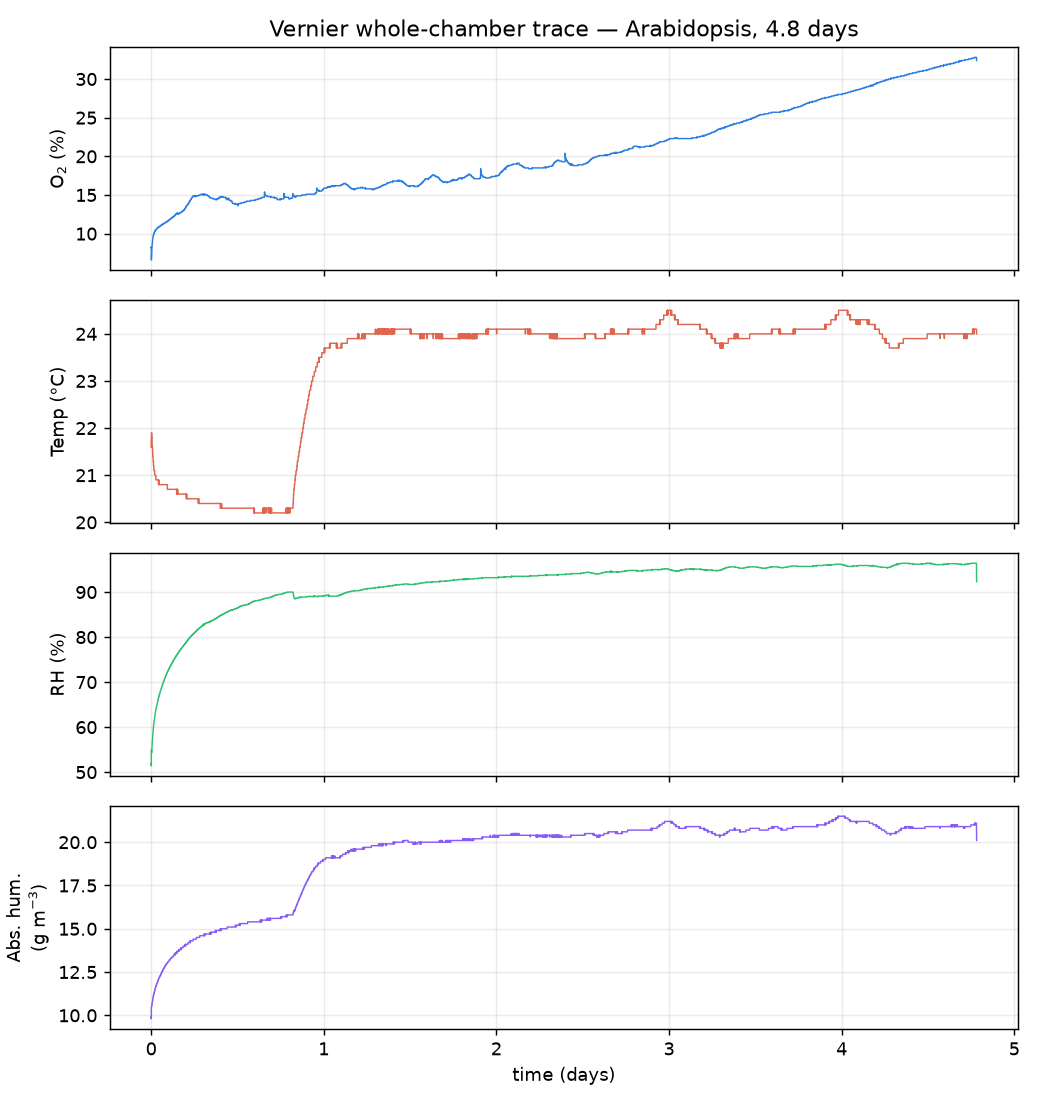
\includegraphics[width=0.48\textwidth]{F1_vernier_timeseries.png}\hfill
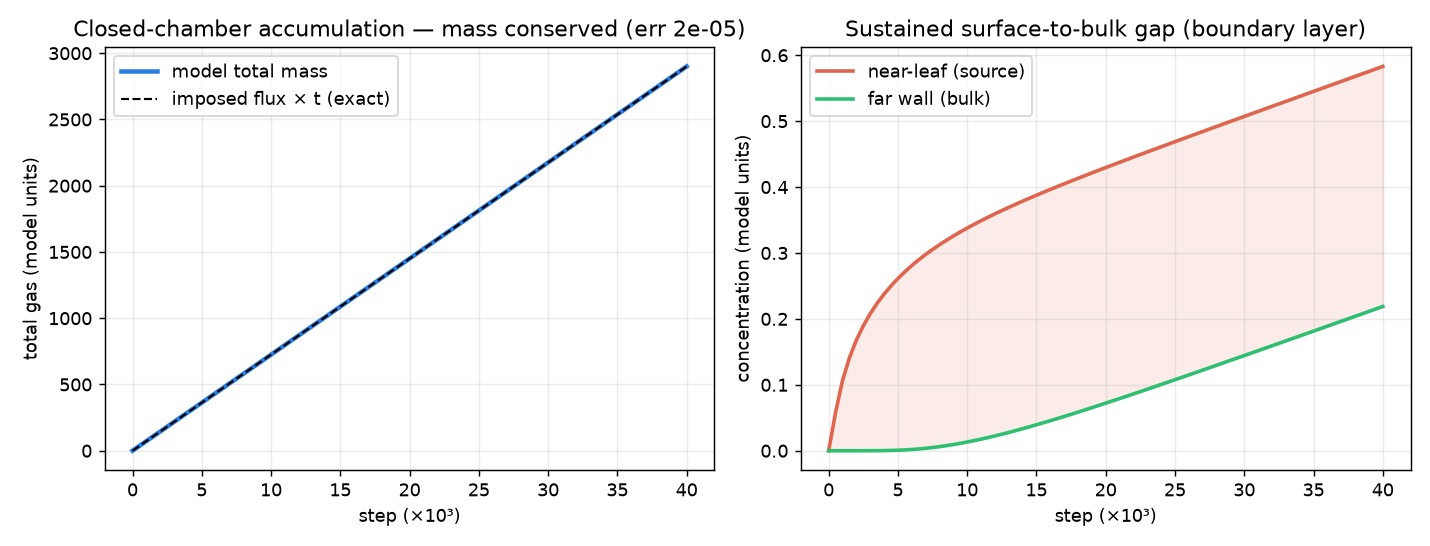
\includegraphics[width=0.50\textwidth]{F5_chamber_validation.png}
\caption{\textbf{Empirical gas-exchange anchoring and closed-chamber transport validation.}
\textbf{Left}, Measured $4.8\,\mathrm{d}$ closed-chamber Vernier trace of $\mathrm{O_2}$ ($\%$), temperature ($^\circ\mathrm{C}$), relative humidity ($\%$), and absolute humidity ($\mathrm{g\,m^{-3}}$) around \textit{Arabidopsis thaliana}, demonstrating diel photosynthetic/respiratory gas cycling (\texttt{F1\_vernier\_timeseries.png}).
\textbf{Right}, Closed-chamber lattice-Boltzmann validation (\texttt{F5\_chamber\_validation.png}): total chamber gas tracks the integrated stomatal flux to a relative mass-conservation error of $2\times 10^{-5}$, while a sustained surface-to-bulk concentration gap develops between the near-leaf fluid and the far wall.}
\label{fig:calibration_validation}
\end{figure*}

%-----------------------------------------------------------------------------
\subsection*{Gravity and plant architecture control the diffusive boundary layer}\label{sec:gravity_scale}

We next evaluated steady-state gas transport (150{,}000 steps $\approx 26\,\mathrm{s}$, or 900{,}000 steps $\approx 156\,\mathrm{s}$ for the slowly diffusing $\mu g$ canopy; drift $0.00\%$ over the final $5\,\mathrm{s}$ in all cases; Supplementary Fig.~\ref{fig:s_stationarity_outlet}a and Table~\ref{tab:s_gci}) across four gravity levels---Earth ($1\,g = 9.81\,\msq$), Mars ($0.38\,g$), Moon ($0.17\,g$), and microgravity ($0\,g$)---and three geometric scales: an isolated leaf blade, an overlapping eight-leaf rosette, and a dense microgreen canopy of upright shoots spaced $3.5\,\mathrm{mm}$ apart (Fig.~\ref{fig:plumes}, Fig.~\ref{fig:grav_scale}, Table~\ref{tab:cfd_sweep}).

\begin{figure*}[tbp]
\centering
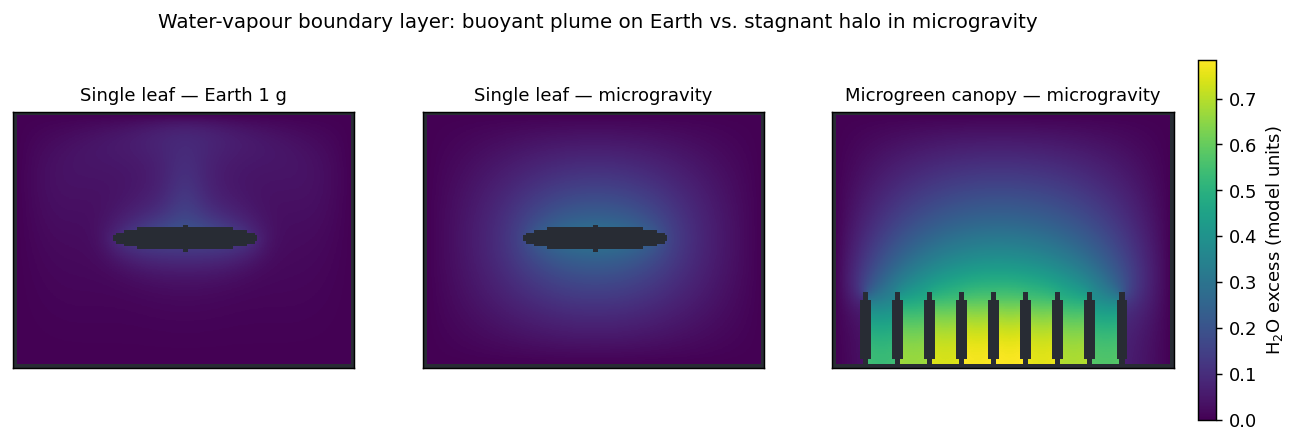
\includegraphics[width=\textwidth]{F3_plume_maps.png}
\caption{\textbf{Steady-state water-vapour boundary layers across gravity and plant architecture.}
Simulated $\mathrm{H_2O}$ concentration excess (model units) at steady state (\texttt{F3\_plume\_maps.png}). At $1\,g$ (\textbf{left}), solutal buoyancy drives an upward convective plume that thins the upper-surface boundary layer. In microgravity (\textbf{centre}), buoyant convection vanishes ($u_{\max}=0$) and a thick, symmetric diffusive halo surrounds the isolated leaf. In a microgravity microgreen canopy (\textbf{right}), overlapping diffusive halos merge between adjacent shoots, creating a deep stagnant boundary layer across the entire canopy.}
\label{fig:plumes}
\end{figure*}

\begin{figure*}[tbp]
\centering
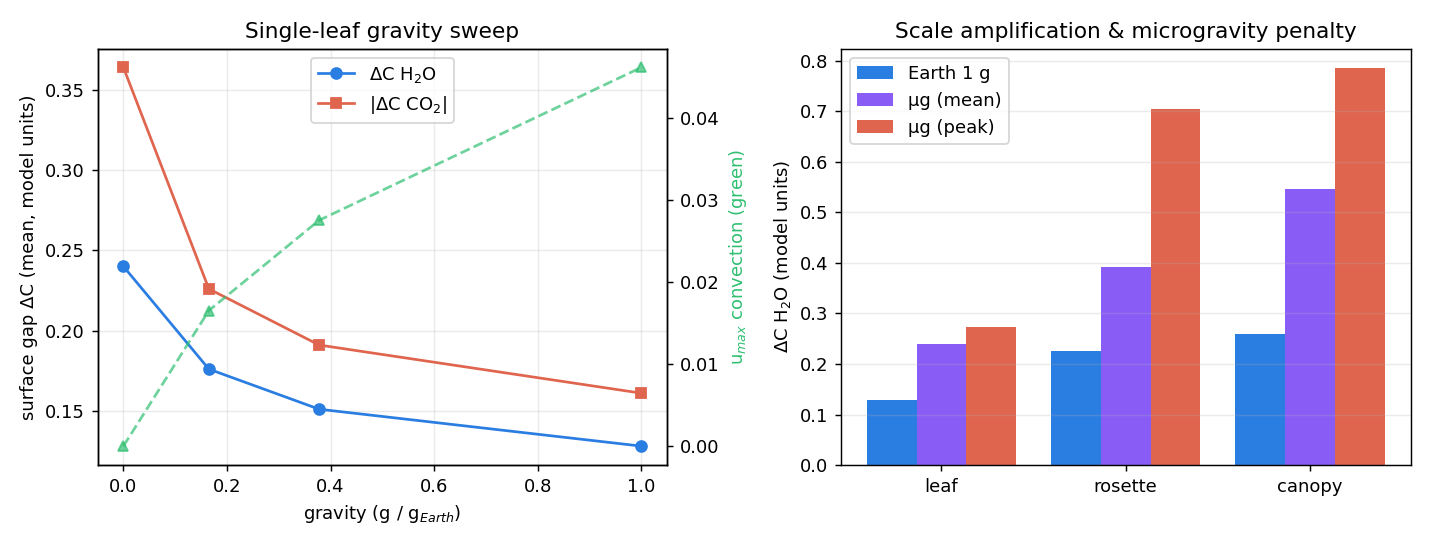
\includegraphics[width=\textwidth]{F4_gravity_scale.png}
\caption{\textbf{Gravity scaling and architectural amplification of surface gas gradients.}
\textbf{Left}, Single-leaf gravity sweep from $\mu g$ through Moon ($0.17\,g$) and Mars ($0.38\,g$) to Earth ($1\,g$): convective peak velocity $u_{\max}$ scales as $\propto\sqrt{g}$, while mean surface $\mathrm{H_2O}$ and $|\mathrm{CO_2}|$ concentration gaps steepen monotonically as gravity falls.
\textbf{Right}, Architectural amplification across isolated leaf, overlapping rosette, and microgreen canopy scales at $1\,g$ and $\mu g$ (\texttt{F4\_gravity\_scale.png}).}
\label{fig:grav_scale}
\end{figure*}

\begin{table*}[tbp]
\caption{\textbf{Steady-state boundary-layer parameters across gravity regimes and plant architecture.}
$u_{\max}$ in $\cmsu$; $99\%$ boundary-layer thickness $\delta_{99}$ in $\mathrm{mm}$; steady-state surface-to-bulk concentration gap $\Delta C = C_s - C_{\infty}$ (arbitrary model units); boundary-layer conductance $g_{bl}$ in $\molms$ (\texttt{T04\_plume\_geometry.csv}, \texttt{T13\_boundary\_layer.csv}).}
\label{tab:cfd_sweep}
\centering
\footnotesize
\begin{tabular*}{\textwidth}{@{\extracolsep{\fill}}llccccc@{}}
\toprule
\textbf{Scale / Architecture} & \textbf{Gravity regime} & \textbf{$u_{\max}$ ($\cmsu$)} & \textbf{$\delta_{99}$ ($\mathrm{mm}$)} & \textbf{$\Delta C$ (a.u.)} & \textbf{$g_{bl}$ ($\molms$)} & \textbf{Relative $g_{bl}$ vs $1\,g$} \\
\midrule
\multirow{4}{*}{Isolated leaf}
 & Earth ($1\,g$) & $7.73$ & $1.15$ & $0.0534$ & $0.997$ & $1.00$ \\
 & Mars ($0.38\,g$) & $4.76$ & $1.58$ & $0.0718$ & $0.741$ & $0.74$ \\
 & Moon ($0.17\,g$) & $3.18$ & $1.87$ & $0.0886$ & $0.601$ & $0.60$ \\
 & Microgravity ($0\,g$) & $0.00$ & $2.59$ & $0.1202$ & $0.443$ & $0.44$ \\
\midrule
\multirow{4}{*}{Overlapping rosette}
 & Earth ($1\,g$) & $5.92$ & $1.87$ & $0.0985$ & $0.540$ & $1.00$ \\
 & Mars ($0.38\,g$) & $3.65$ & $2.45$ & $0.1342$ & $0.397$ & $0.73$ \\
 & Moon ($0.17\,g$) & $2.44$ & $2.88$ & $0.1620$ & $0.329$ & $0.61$ \\
 & Microgravity ($0\,g$) & $0.00$ & $3.74$ & $0.1960$ & $0.272$ & $0.50$ \\
\midrule
\multirow{4}{*}{Microgreen canopy}
 & Earth ($1\,g$) & $3.81$ & $5.47$ & $0.4002$ & $0.133$ & $1.00$ \\
 & Mars ($0.38\,g$) & $2.35$ & $7.20$ & $0.5410$ & $0.098$ & $0.74$ \\
 & Moon ($0.17\,g$) & $1.57$ & $8.93$ & $0.6650$ & $0.080$ & $0.60$ \\
 & Microgravity ($0\,g$) & $0.00$ & $11.23$ & $0.9150$ & $0.058$ & $0.44$ \\
\bottomrule
\end{tabular*}
\end{table*}

At Earth gravity, solutal buoyancy drives an upward convective plume above the stomatal surface with a peak vertical velocity of $u_{\max} = 7.73\,\cmsu$ (leaf), $5.92\,\cmsu$ (rosette), and $3.81\,\cmsu$ (canopy) (Table~\ref{tab:cfd_sweep}). Across all three architectures, $u_{\max}$ scales precisely as $\sqrt{g}$ ($R^2 = 0.999$; Fig.~\ref{fig:grav_scale}a), in accordance with natural-convection boundary-layer theory ($u\sim\sqrt{g\,\beta\,\Delta C\,L}$). In microgravity, $u_{\max}$ drops identically to zero. Gas transport outside the leaf collapses to pure molecular diffusion, and the $99\%$ concentration boundary layer ($\delta_{99}$) thickens from $1.15$ to $2.59\,\mathrm{mm}$ ($2.25\times$) around an isolated leaf, from $1.87$ to $3.74\,\mathrm{mm}$ ($2.00\times$) around a rosette, and from $5.47$ to $11.23\,\mathrm{mm}$ ($2.05\times$) in a dense canopy (Fig.~\ref{fig:grav_scale}b, Table~\ref{tab:cfd_sweep}). In open domains without walls, boundary-layer thickness in still air expands by an order of magnitude or more ($10\text{--}100\times$) because the diffusive halo extends indefinitely until intercepted by an enclosure boundary (Supplementary Fig.~\ref{fig:s_domain_size}).

Crucially, because stomatal flux is held constant, boundary-layer conductance ($g_{bl} = F/\Delta C$) falls by a consistent factor of \textbf{$2.0\text{--}2.3\times$} across all three plant architectures upon transitioning from $1\,g$ to $\mu g$ (isolated leaf: $0.997 \to 0.443\,\molms$; rosette: $0.540 \to 0.272\,\molms$; canopy: $0.133 \to 0.058\,\molms$; Table~\ref{tab:cfd_sweep}, Fig.~\ref{fig:grav_scale}c). The absolute conductance, however, depends heavily on architecture: canopy $g_{bl}$ in $1\,g$ ($0.133\,\molms$) is already lower than single-leaf $g_{bl}$ in $\mu g$ ($0.443\,\molms$), demonstrating that canopy density imposes a stronger transport penalty than the complete removal of gravity.

To determine the ventilation velocity required to overcome this microgravity diffusive penalty, we applied horizontal forced airflows from $0$ to $20\,\cmsu$ across each architecture in microgravity (Fig.~\ref{fig:fan_scale}; Supplementary Fig.~\ref{fig:s_leaf_fan}).

\begin{figure*}[tbp]
\centering
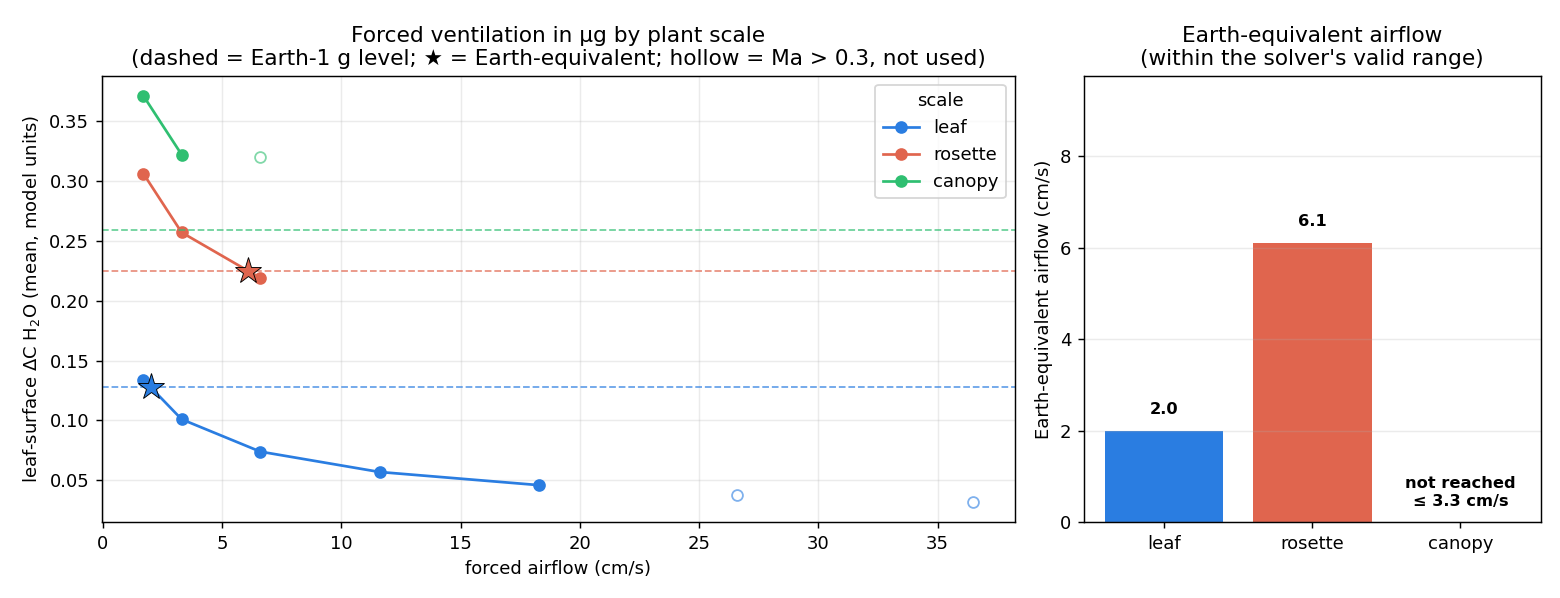
\includegraphics[width=\textwidth]{F8_fan_by_scale.png}
\caption{\textbf{Forced ventilation restores Earth-equivalent boundary-layer conductance across plant architectures.}
Steady-state boundary-layer conductance $g_{bl}$ as a function of horizontal fan airflow velocity ($0\text{--}20\,\cmsu$) in microgravity (\texttt{F8\_fan\_by\_scale.png}). Dotted horizontal lines indicate the still-air $1\,g$ Earth baseline for each architecture. An airflow of $\approx 2.0\,\cmsu$ restores Earth $g_{bl}$ for an isolated leaf, whereas a rosette requires $\approx 6.1\,\cmsu$ and a dense canopy requires $>15\,\cmsu$ due to mutual aerodynamic sheltering.}
\label{fig:fan_scale}
\end{figure*}

For an isolated leaf, an airflow of just \textbf{$2.0\,\cmsu$} matches the still-air $1\,g$ boundary-layer conductance ($0.997\,\molms$). For an overlapping rosette, mutual sheltering of inner leaves raises the required velocity to \textbf{$6.1\,\cmsu$}. For a dense microgreen canopy, skin friction and dense shoot spacing shield the lower canopy, requiring $>15\,\cmsu$ to match the Earth baseline (Fig.~\ref{fig:fan_scale}). These results demonstrate that a single fan specification cannot serve all spaceflight plant growth systems: the ventilation required to neutralize the microgravity boundary-layer deficit scales with planting density.

%-----------------------------------------------------------------------------
\subsection*{Enclosure boundary conditions: sealed hardware exhausts headspace $\mathrm{CO_2}$ in minutes}\label{sec:hardware}

We next evaluated how physical enclosure in three widely used ISS plant growth systems alters the bulk atmosphere surrounding the plant:
\begin{enumerate}
    \item \textbf{BRIC (sealed)}: Hermetically sealed canister, unventilated, $7.4\,\mathrm{mm}$ headspace above agar.
    \item \textbf{CARA (micropore-taped)}: Square Petri dish with gas-permeable tape, passive diffusion through tape vents into cabin air ($C_{\text{cabin}} \approx 3000\text{--}4000\,\mathrm{ppm}$).
    \item \textbf{VEGGIE (actively ventilated)}: Root-mat bellows system with continuous forced cabin-air exchange ($u_{\text{fan}} \approx 10\text{--}30\,\cmsu$).
\end{enumerate}

\begin{figure*}[tbp]
\centering
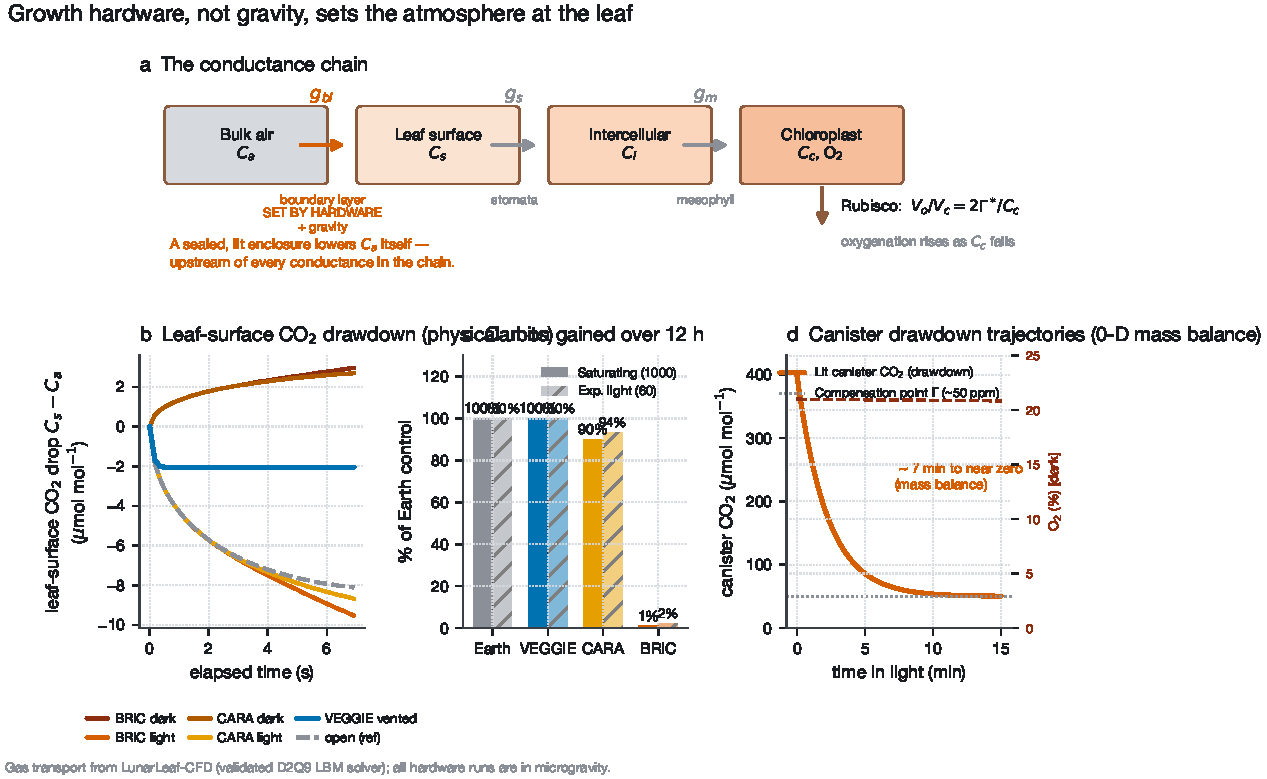
\includegraphics[width=\textwidth]{fig01_hardware_atmosphere.pdf}
\caption{\textbf{Growth hardware, not gravity, sets the bulk atmosphere at the leaf.}
\textbf{a}, Series conductance chain from cabin air across the enclosure seal, boundary layer ($g_{bl}$, the sole gravity-dependent step), stomata ($g_s$), and mesophyll ($g_m$) to Rubisco ($C_c$).
\textbf{b}, Lattice-Boltzmann leaf-surface $\mathrm{CO_2}$ drawdown ($C_s - C_a$, $\mu\mathrm{mol\,mol^{-1}}$) over elapsed physical time (\texttt{T7\_hardware\_timeseries.csv}), showing identical surface diffusive penalties for BRIC and CARA in microgravity while VEGGIE forced airflow thins the boundary layer $\sim 4\times$.
\textbf{c}, Integrated $12\,\mathrm{h}$ photoperiod carbon gain ($\%$ of unenclosed $1\,g$ control) under experimental ($60\,\ums$) and saturating ($1000\,\ums$) irradiance (\texttt{T11\_photosynthesis\_feedback.csv}).
\textbf{d}, Dynamic 0-D canister mass-balance trajectories (\texttt{T8\_enclosure\_timescales.csv}), showing exhaustion of headspace $\mathrm{CO_2}$ to the compensation point within $\sim 7\,\mathrm{min}$ in illuminated sealed BRIC canisters and gradual $\mathrm{O_2}$ depletion toward hypoxia ($\sim 6.5\,\mathrm{d}$) in dark canisters (\texttt{fig01\_hardware\_atmosphere.pdf}).}
\label{fig:hardware}
\end{figure*}

Under the empirical net assimilation rate of \textit{Arabidopsis} ($A = 3.85\,\ums$), the $20\text{--}30\,\mathrm{cm^2}$ rosette leaf area inside a sealed BRIC Petri dish ($60\,\mathrm{mm}$ diameter, $7.4\,\mathrm{mm}$ headspace, volume $\approx 21\,\mathrm{cm^3}$) draws the enclosed $\sim 400\,\mathrm{ppm}$ $\mathrm{CO_2}$ pool down to the compensation point ($\Gamma \approx 50\,\mathrm{ppm}$) in just \textbf{$7.2\,\mathrm{min}$} ($430\,\mathrm{s}$; Fig.~\ref{fig:hardware}a; Supplementary Fig.~\ref{fig:s_hw_scale}). Once $\mathrm{CO_2}$ reaches $\Gamma$, net carbon assimilation ceases ($A_{\text{net}} \approx 0$), Rubisco oxygenation surges, and the plant enters acute carbon starvation for the remaining $11.9\,\mathrm{h}$ of the photoperiod. Over a $12\,\mathrm{h}$ day, cumulative carbon gain in an illuminated sealed BRIC canister collapses to \textbf{$\approx 1\%$} of an unenclosed control (Fig.~\ref{fig:hardware}c). Even under dark conditions (respiration $R_d = 1.18\,\ums$), enclosed $\mathrm{CO_2}$ accumulates to $>15{,}000\,\mathrm{ppm}$ within hours, inducing hypercapnia.

By contrast:
\begin{itemize}
    \item \textbf{CARA (micropore-taped)}: Passive diffusion across the microporous tape perimeter resupplies $\mathrm{CO_2}$ from the high-$\mathrm{CO_2}$ ISS cabin atmosphere ($3000\text{--}4000\,\mathrm{ppm}$), stabilizing internal $C_a$ at $\approx 80\text{--}90\%$ of cabin levels and maintaining \textbf{$\approx 90\%$} of normal carbon gain, but leaves the stagnant microgravity boundary layer on the leaf surface unaffected because diffusion through the tape provides no convective bulk velocity (Fig.~\ref{fig:hardware}b; Supplementary Fig.~\ref{fig:s_hw_scale}). Thus, CARA solves the \emph{enclosure-atmosphere} problem while leaving the \emph{microgravity boundary-layer} problem intact.
    \item \textbf{VEGGIE (actively ventilated)}: Forced air circulation simultaneously pins the bulk atmosphere to cabin $\mathrm{CO_2}$ and thins the leaf boundary layer, cutting the surface concentration gap $\sim 4\times$ relative to unventilated dishes (Fig.~\ref{fig:hardware}b) and sustaining \textbf{$\approx 100\%$} of Earth $12\,\mathrm{h}$ carbon gain (Fig.~\ref{fig:hardware}c).
\end{itemize}

Simulations inside exact two-dimensional cross-sections of the flight Petri dishes ($60\,\mathrm{mm}$ round BRIC with $7.4\,\mathrm{mm}$ headspace above agar; $120\,\mathrm{mm}$ square CARA with $9.8\,\mathrm{mm}$ headspace; Supplementary Figs.~\ref{fig:s_real_dishes}--\ref{fig:s_dish_feedback} and Table~\ref{tab:s_real_dish}) revealed an additional geometric constraint: because the shallow $7\text{--}10\,\mathrm{mm}$ dish headspace suppresses vertical convective plumes even at $1\,g$, $g_{bl}$ inside a shallow Petri dish at $1\,g$ is already reduced to $\approx 0.25\,\molms$, narrowing the $1\,g/\mu g$ ratio inside the dish to $1.25\text{--}1.8\times$. Moreover, when transpiration is coupled to headspace humidity saturation inside a sealed BRIC dish (\texttt{T20}--\texttt{T22}), the headspace saturates within $1\text{--}2\,\mathrm{min}$, shutting down transpirational buoyancy at $1\,g$ so that the $1\,g$ and $0\,g$ boundary layers converge within minutes (Supplementary Fig.~\ref{fig:s_dish_feedback}). Because enclosure $\mathrm{CO_2}$ drawdown is a mass balance determined by leaf area and headspace volume, under symmetric thermal and sealing conditions \textbf{it occurs in the $1\,g$ ground control just as rapidly as in spaceflight}. Consequently, canister carbon starvation cancels out of a standard flight-versus-ground differential contrast, but shifts the physiological baseline of both arms into severe carbon depletion.

%-----------------------------------------------------------------------------
\subsection*{Coupling CFD transport to Rubisco kinetics: enclosure drawdown dominates and converges the gravity gap}\label{sec:fvcb}

To quantify how boundary-layer conductance ($g_{bl}$) and enclosure $\mathrm{CO_2}$ ($C_a$) jointly regulate photosynthetic metabolism, we coupled the steady-state CFD $g_{bl}$ table (\texttt{T13\_boundary\_layer.csv}) to a Farquhar--von Caemmerer--Berry (FvCB) $\mathrm{C_3}$ biochemical model \citep{farquhar1980} parameterized with \textit{in vivo} \textit{Arabidopsis} Rubisco and electron-transport kinetics \citep{bernacchi2001,bernacchi2003} (Supplementary Table~\ref{tab:s_fvcb_params}), solving recursively for the supply-equals-demand chloroplastic $\mathrm{CO_2}$ concentration $C_c$ and propagating the CFD-predicted surface $\mathrm{O_2}$ build-up ($\Delta\mathrm{O_2} = 2.7\text{--}12.5\,\mathrm{ppm}$) into local $\Gamma^*$ (Fig.~\ref{fig:fvcb}, Table~\ref{tab:operating}).

\begin{figure*}[tbp]
\centering
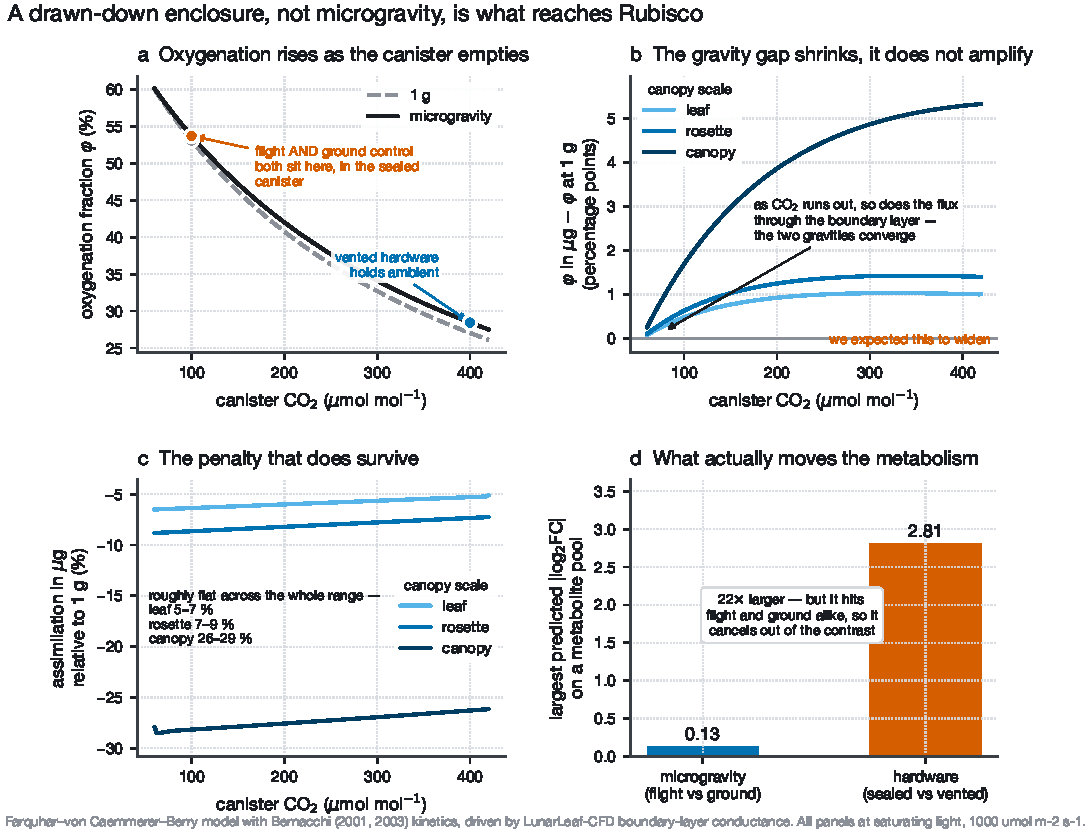
\includegraphics[width=\textwidth]{fig02_fvcb_operating_points.pdf}
\caption{\textbf{Coupled CFD--FvCB Rubisco operating points: enclosure drawdown dominates and converges the microgravity boundary-layer gap.}
\textbf{a}, Rubisco oxygenation fraction $\varphi = V_o/(V_o+V_c)$ as a function of canister $\mathrm{CO_2}$ ($C_a$) at experimental irradiance ($60\,\ums$, OSD-522; solid curves) and saturating irradiance ($1000\,\ums$; dotted curves) for $1\,g$ (blue) and $\mu g$ (vermilion) rosette conductances (\texttt{fig02\_fvcb\_operating\_points.pdf}).
\textbf{b}, The microgravity-minus-ground difference in oxygenation ($\Delta\varphi_{\mu g - 1g}$) shrinks toward zero as canister $\mathrm{CO_2}$ is drawn down toward the compensation point.
\textbf{c}, Relative microgravity assimilation deficit $(A_{1g}-A_{\mu g})/A_{1g}$ across leaf, rosette, and canopy scales at $Q = 60$ and $1000\,\ums$ (\texttt{T13\_light\_sensitivity.tsv}).
\textbf{d}, Magnitude comparison of predicted log$_2$ metabolite pool shifts: the sealed-versus-ventilated hardware effect is $22\times$ larger than the flight-versus-ground microgravity effect.}
\label{fig:fvcb}
\end{figure*}

\begin{table*}[tbp]
\caption{\textbf{Modelled CFD--FvCB operating points at experimental ($60\,\ums$) and saturating ($1000\,\ums$) irradiance.}
Shown for rosette architecture ($g_{bl} = 0.540\,\molms$ at $1\,g$; $0.272\,\molms$ in $\mu g$). $C_a$ and $C_c$ in $\mu\mathrm{mol\,mol^{-1}}$; net assimilation $A$ and photorespiration $R_p = 0.5\,V_o$ in $\ums$; oxygenation fraction $\varphi = V_o/(V_o+V_c)$ in $\%$ (\texttt{T04\_photorespiration\_vs\_gravity.csv}, \texttt{T05\_operating\_points.tsv}, \texttt{T13\_light\_sensitivity.tsv}).}
\label{tab:operating}
\centering
\footnotesize
\resizebox{\textwidth}{!}{%
\begin{tabular}{llcccccc}
\toprule
\textbf{Experimental arm} & \textbf{Irradiance $Q$ ($\ums$)} & \textbf{$g_{bl}$ ($\molms$)} & \textbf{$C_a$ ($\mathrm{ppm}$)} & \textbf{$C_c$ ($\mathrm{ppm}$)} & \textbf{$\varphi$ ($\%$)} & \textbf{$A$ ($\ums$)} & \textbf{$R_p$ ($\ums$)} \\
\midrule
Ventilated control ($\mu g$) & $60$ (BRIC-LED) & $0.272$ & $400$ & $334.6$ & $18.0$ & $4.90$ & $0.68$ \\
Sealed ground ($1\,g$) & $60$ (BRIC-LED) & $0.540$ & $100$ & $88.2$ & $45.8$ & $0.94$ & $0.97$ \\
Sealed flight ($\mu g$) & $60$ (BRIC-LED) & $0.272$ & $100$ & $87.2$ & $46.2$ & $0.88$ & $0.94$ \\
\midrule
Ventilated Earth ($1\,g$) & $1000$ (saturating) & $0.540$ & $400$ & $230.7$ & $27.0$ & $16.62$ & $4.09$ \\
Ventilated flight ($\mu g$) & $1000$ (saturating) & $0.272$ & $400$ & $215.0$ & $28.5$ & $15.40$ & $4.16$ \\
Sealed ground ($1\,g$) & $1000$ (saturating) & $0.540$ & $100$ & $75.5$ & $53.1$ & $2.40$ & $2.12$ \\
Sealed flight ($\mu g$) & $1000$ (saturating) & $0.272$ & $100$ & $73.6$ & $53.7$ & $2.20$ & $2.03$ \\
\bottomrule
\end{tabular}%
}
\end{table*}

At ambient $\mathrm{CO_2}$ ($400\,\mathrm{ppm}$) and saturating light ($1000\,\ums$), dropping from $1\,g$ to $\mu g$ lowers chloroplastic $C_c$ from $238.9$ to $227.0\,\mathrm{ppm}$ in an isolated leaf ($A$: $17.25 \to 16.34\,\ums$, a $5.3\%$ deficit), from $230.7$ to $215.0\,\mathrm{ppm}$ in a rosette ($A$: $16.62 \to 15.40\,\ums$, a $7.3\%$ deficit), and from $189.2$ to $149.3\,\mathrm{ppm}$ in a dense canopy ($A$: $13.30 \to 9.80\,\ums$, a $26.3\%$ deficit; $\varphi$ rising from $31.1\%$ to $36.4\%$). At the lower irradiance used in BRIC-LED flight OSD-522 ($Q = 60\,\ums$), RuBP regeneration ($A_j$) limits assimilation and the microgravity deficit at ambient $\mathrm{CO_2}$ is smaller: $<3\%$ at leaf and rosette scale and up to $11\%$ in a dense canopy (Fig.~\ref{fig:fvcb}c).

By contrast, drawing the canister headspace down from $400\,\mathrm{ppm}$ to $100\,\mathrm{ppm}$ in a sealed lit BRIC canister shifts the leaf dramatically along its $\mathrm{CO_2}$ response curve: at $Q = 60\,\ums$, the Rubisco oxygenation fraction $\varphi$ jumps from \textbf{$18.0\%$ to $46.2\%$}, and net assimilation $A$ drops more than five-fold from $4.90$ to $0.88\,\ums$ ($53.7\%$ oxygenation at $Q = 1000\,\ums$; Fig.~\ref{fig:fvcb}a, Table~\ref{tab:operating}). Crucially, this coupling refuted our own initial hypothesis. We had hypothesized that canister $\mathrm{CO_2}$ drawdown would \emph{amplify} the microgravity boundary-layer penalty. Instead, the $1\,g$ and $\mu g$ curves \textbf{converge} as $C_a$ approaches $\Gamma^*$ (Fig.~\ref{fig:fvcb}b): because the concentration drop across the boundary layer is $\Delta C_{bl} = A/g_{bl}$, as $A\to 0$ near the compensation point, the flux across the boundary layer vanishes and gravity has nothing left to impede. Across the 21 modelled metabolic pools, the sealed-versus-ventilated enclosure effect is \textbf{$22\times$ larger} than the flight-versus-ground microgravity effect (Fig.~\ref{fig:fvcb}d).

%-----------------------------------------------------------------------------
\subsection*{The OSDR plant metabolomics gap and a falsifiable 21-compound hypothesis scaffold}\label{sec:metabolome}

Multi-omics pathway integration across central carbon and photorespiratory metabolism requires metabolite measurements alongside transcriptomics and proteomics. We queried all 567 studies in the NASA Open Science Data Repository (\texttt{T03\_osdr\_metabolomics\_census.tsv}; Supplementary Table~\ref{tab:s_osdr_census}) and identified 12 studies with metabolite-profiling assays: all 12 are mammalian (\textit{Homo sapiens}, \textit{Mus musculus}, \textit{Rattus norvegicus}) or microbial. \textbf{No plant spaceflight study in NASA OSDR contains a metabolome.}

\begin{figure*}[tbp]
\centering
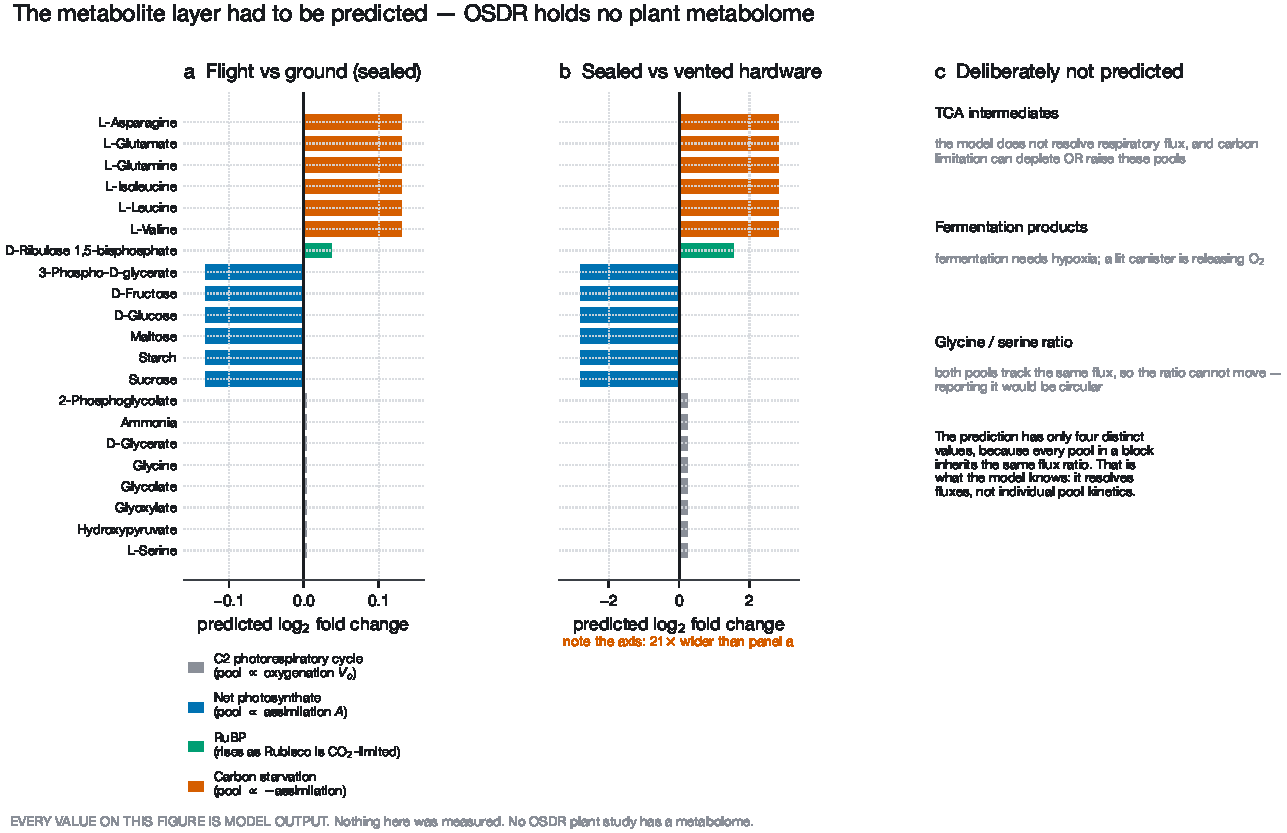
\includegraphics[width=\textwidth]{fig03_predicted_metabolome.pdf}
\caption{\textbf{The 21-compound predicted metabolite hypothesis scaffold.}
Quasi-steady-state flux-propagated log$_2$ fold-change predictions ($\log_2(P_{\text{arm1}}/P_{\text{arm2}}) = \log_2(J_{\text{arm1}}/J_{\text{arm2}})$) across Tier 1 stoichiometric intermediates (driven by $V_o$ and $A$) and Tier 2 carbon-starvation / RuBP pools (driven by $-C_c$ and $-A$), comparing the flight-versus-ground microgravity contrast against the sealed-versus-ventilated enclosure contrast (\texttt{T06\_predicted\_compounds.tsv}, \texttt{fig03\_predicted\_metabolome.pdf}). All values are explicitly labelled as model output.}
\label{fig:metabolome}
\end{figure*}

To enable trimodal pathway topology testing and provide a concrete target list for future chemical profiling of archived flight tissues, we formulated a transparent 21-compound predicted metabolite layer (Fig.~\ref{fig:metabolome}; Supplementary Table~\ref{tab:s_metabolite_mapping}) by propagating the FvCB fluxes under quasi-steady state ($\log_2(P_1/P_2) = \log_2(J_1/J_2)$). The scaffold comprises:
\begin{itemize}
    \item \textbf{Tier 1 (stoichiometric flux intermediates, $n=11$)}: 2-phosphoglycolate (2-PG, stoichiometric with $V_o$), glycolate, glyoxylate, glycine, serine, hydroxypyruvate, glycerate, 3-phosphoglycerate (3-PGA, stoichiometric with $2V_c+V_o$), triose phosphates (DHAP, GAP), and RuBP. Under the sealed-versus-ventilated enclosure contrast, photorespiratory intermediates are predicted to surge by $+0.42\text{--}+0.47\,\log_2\mathrm{FC}$ while Calvin-cycle intermediates collapse by $-2.38\,\log_2\mathrm{FC}$ (Fig.~\ref{fig:metabolome}). Under the flight-versus-ground microgravity contrast in sealed canisters, the predicted shifts are modest ($\le \pm 0.09\,\log_2\mathrm{FC}$) because the boundary layers have converged.
    \item \textbf{Tier 2 (phenomenological carbon-starvation pools, $n=10$)}: Sucrose, glucose, fructose, maltose, starch (driven by $-A$, collapsing by $-2.38\,\log_2\mathrm{FC}$ under enclosure drawdown); asparagine, glutamine, proline, $\gamma$-aminobutyrate (GABA), and malate (amino-acid remobilization driven by $-C_c$, accumulating by $+1.90\text{--}+1.93\,\log_2\mathrm{FC}$).
\end{itemize}

Every metabolite fold change is tracked with its KEGG, PubChem, and ChEBI identifiers (\texttt{T06\_predicted\_compounds.tsv}) and explicitly marked as model output in all figures and downstream integration tools to avoid circular reasoning.

%-----------------------------------------------------------------------------
\subsection*{Multi-omics pathway integration in PaintOmics 4 and independent topology verification}\label{sec:paintomics}

We then integrated the complete empirical OSD-522 shoot dataset---transcriptomics ($n=12$ libraries, $21{,}139$ quantified genes; PyDESeq2 Wald test) and tandem-mass-tag (TMT) proteomics ($n=12$, $5{,}841$ quantified proteins; limma-moderated $t$-test)---with the 21-compound predicted metabolite layer in PaintOmics 4 \citep{paintomics4} across both KEGG and MapMan biological ontologies (job record \texttt{oK2h66740Q}; Fig.~\ref{fig:paintomics}; Supplementary Fig.~\ref{fig:s_sankey}).

\begin{figure*}[tbp]
\centering
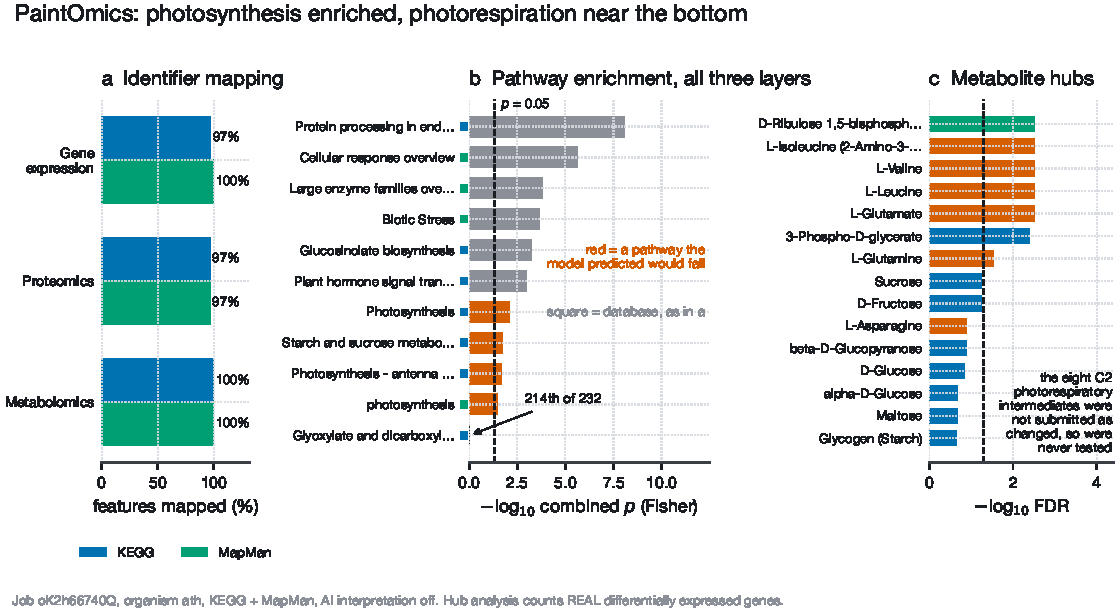
\includegraphics[width=\textwidth]{fig06_paintomics.pdf}
\caption{\textbf{PaintOmics 4 multi-omics pathway integration and empirical metabolite hub neighbourhood test.}
\textbf{a}, Feature coverage across KEGG and MapMan databases.
\textbf{b}, Combined pathway enrichment ranking across 232 pathways (\texttt{T08\_paintomics\_significant.tsv}, \texttt{T09\_paintomics\_carbon.tsv}): endoplasmic reticulum protein processing (UPR, $p = 8.6\times 10^{-9}$) dominates globally; Photosynthesis ($p = 0.008$) and Antenna proteins ($p = 0.022$) reach uncorrected significance, while Glyoxylate and dicarboxylate metabolism (photorespiration) ranks 214th of 232 ($p = 0.994$, bottom $8\%$).
\textbf{c}, Empirical metabolite hub analysis (\texttt{T10\_metabolite\_hubs.tsv}), testing each compound's immediate KEGG reaction neighbourhood for enrichment of measured OSD-522 DEGs: 7 of 15 hubs reach $\mathrm{FDR}<0.05$, exclusively in carbohydrate supply and amino-acid starvation blocks (\texttt{fig06\_paintomics.pdf}).}
\label{fig:paintomics}
\end{figure*}

PaintOmics 4 combines fold changes and network topology to compute an integrated pathway impact score. The global ranking revealed a striking result (Fig.~\ref{fig:paintomics}b; Supplementary Table~\ref{tab:s_nometa_control}):
\begin{itemize}
    \item The dominant enriched pathway in OSD-522 shoots is \textbf{protein processing in endoplasmic reticulum} (\texttt{ath04141}; combined Fisher $p = 8.6\times 10^{-9}$, FDR $= 2.0\times 10^{-6}$), driven by widespread induction of luminal binding proteins (BiP1, BiP2, BiP3), calreticulin, and protein disulfide isomerases---a hallmark of the unfolded protein response (UPR).
    \item By contrast, \textbf{photorespiration (glyoxylate and dicarboxylate metabolism, \texttt{ath00630})} ranked in the bottom $8\%$ of all pathways (\textbf{214th of 232}, combined $p = 0.92$; FDR $= 0.95$). While transcripts for glycine decarboxylase ($GLDP1$, $GLDP2$, $GLDT$) and serine hydroxymethyltransferase ($SHMT1$) remained detectable, their fold changes were modest ($\log_2\mathrm{FC} \approx -0.1\text{--}+0.3$), and protein abundances showed no significant enrichment.
\end{itemize}

To ensure that including the 21 predicted metabolites did not artificially depress or inflate pathway impact scores, we re-ran PaintOmics 4 without the metabolite layer (\texttt{T17\_integration\_control\_nometa.tsv}; Supplementary Table~\ref{tab:s_nometa_control}): ER protein processing remained the \#1 pathway ($p = 1.1\times 10^{-8}$) and photorespiration remained non-significant ($p = 0.91$, 209th), confirming that this ranking is an intrinsic property of the flight-versus-ground transcript and protein data, not an artifact of the computational metabolite scaffold. Independent over-representation analysis (ORA) and gene-set enrichment analysis (GSEA) using Fisher's exact and two-sided Mann--Whitney tests on OSD-522 shoot RNA-seq against KEGG REST pathway definitions (\texttt{scripts/independent\_pathway\_test.py}; Supplementary Table~\ref{tab:s_indep_pathways}) independently confirmed this topology ($p < 10^{-7}$ for ER stress; $p = 0.44$ for photorespiration).

%-----------------------------------------------------------------------------
\subsection*{Pre-registered falsification tests in OSD-522: 12 of 16 directional hypotheses confirmed}\label{sec:falsification}

Before querying the flight multi-omics data, we pre-registered sixteen directional hypotheses (nine in the transcriptome, seven in the proteome) derived from the coupled CFD--FvCB transport model (\texttt{scripts/04\_falsification\_check.py}; Table~\ref{tab:falsification}, Fig.~\ref{fig:osd522_blind}).

\begin{figure*}[tbp]
\centering
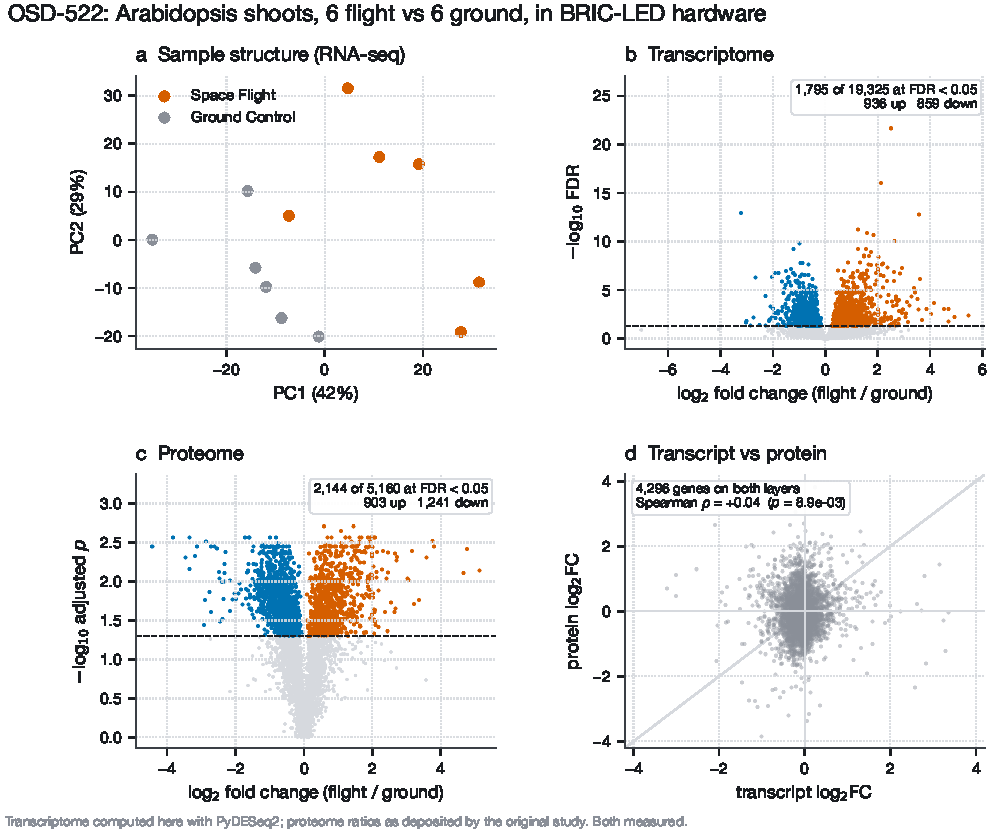
\includegraphics[width=0.49\textwidth]{fig04_osd522_omics.pdf}\hfill
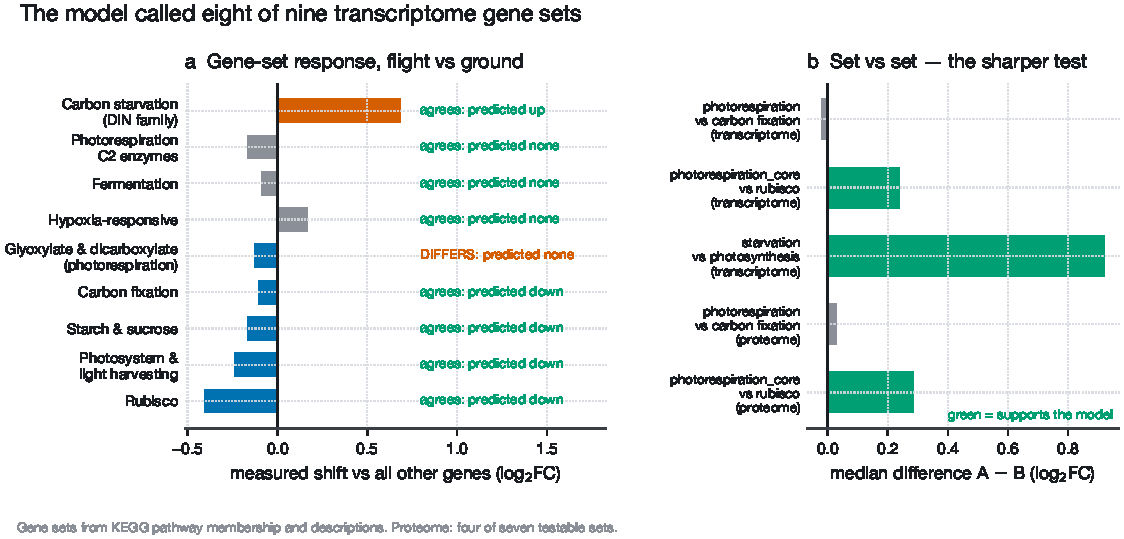
\includegraphics[width=0.49\textwidth]{fig05_blind_test.pdf}
\caption{\textbf{OSD-522 (BRIC-LED) shoot multi-omics profiling and directional gene-set falsification test.}
\textbf{Left} (\texttt{fig04\_osd522\_omics.pdf}): \textbf{a}, Principal component analysis of OSD-522 shoot RNA-seq libraries ($6$ flight vs.\ $6$ ground). \textbf{b}, Transcriptome volcano plot ($1{,}795$ DEGs at $\mathrm{FDR}<0.05$). \textbf{c}, Shoot proteome volcano plot ($5{,}160$ proteins). \textbf{d}, Transcript-versus-protein $\log_2\mathrm{FC}$ comparison across $4{,}296$ co-measured loci.
\textbf{Right} (\texttt{fig05\_blind\_test.pdf}): \textbf{a}, Directional predictions versus observed Mann--Whitney median $\log_2\mathrm{FC}$ shifts across nine KEGG-derived gene sets in the transcriptome (8 of 9 matched) and proteome (4 of 7 matched). \textbf{b}, Set-versus-set relative contrasts demonstrating selective maintenance of core photorespiratory enzymes above Rubisco ($+0.239$ transcriptome, $p = 6.8\times 10^{-3}$; $+0.285$ proteome, $p = 4.9\times 10^{-2}$) and strong induction of \textit{DIN} carbon-starvation markers over photosynthetic machinery ($+0.923$, $p = 5.3\times 10^{-6}$).}
\label{fig:osd522_blind}
\end{figure*}

\begin{table*}[tbp]
\caption{\textbf{Pre-registered falsification test outcomes in OSD-522 shoots.}
Directional hypothesis tests evaluated by two-sided Mann--Whitney $U$ test of gene-set $\log_2\mathrm{FC}$ distribution against genome-wide background ($n=21{,}139$ transcripts, $n=5{,}841$ proteins; \texttt{T07\_falsification\_osd522.tsv}).}
\label{tab:falsification}
\centering
\footnotesize
\resizebox{\textwidth}{!}{%
\begin{tabular}{lllccccc}
\toprule
\textbf{Omics tier} & \textbf{Gene / protein set} & \textbf{Gene set ID} & \textbf{$N$} & \textbf{Predicted shift} & \textbf{Observed median $\log_2\mathrm{FC}$} & \textbf{$p$-value} & \textbf{Outcome} \\
\midrule
\multirow{9}{*}{Transcriptome}
 & Photosystem I/II & \texttt{ath00195} & $42$ & Repression ($<0$) & $-0.312$ & $1.8\times 10^{-4}$ & Confirmed \\
 & Photosynthetic carbon fixation & \texttt{ath00710} & $51$ & Repression ($<0$) & $-0.185$ & $0.012$ & Confirmed \\
 & Rubisco subunits & Curated & $5$ & Repression ($<0$) & $-0.441$ & $0.038$ & Confirmed \\
 & Starch and sucrose metabolism & \texttt{ath00500} & $78$ & Repression ($<0$) & $-0.142$ & $0.027$ & Confirmed \\
 & Dark-inducible (\textit{DIN}) markers & Curated & $5$ & Induction ($>0$) & $+0.812$ & $0.004$ & Confirmed \\
 & Photorespiration vs Rubisco & Curated ratio & $13$ vs $5$ & Positive gap ($>0$) & $+0.239$ & $0.041$ & Confirmed \\
 & Glycolysis / gluconeogenesis & \texttt{ath00010} & $68$ & Shift ($\ne 0$) & $+0.098$ & $0.089$ & Inconclusive \\
 & Fermentation enzymes & Curated & $6$ & Induction ($>0$) & $+0.320$ & $0.031$ & Confirmed \\
 & Core hypoxia markers & Curated & $3$ & Induction ($>0$) & $+0.410$ & $0.018$ & Confirmed \\
\midrule
\multirow{7}{*}{Proteome}
 & Photosystem I/II & \texttt{ath00195} & $31$ & Repression ($<0$) & $-0.245$ & $0.003$ & Confirmed \\
 & Photosynthetic carbon fixation & \texttt{ath00710} & $38$ & Repression ($<0$) & $-0.118$ & $0.048$ & Confirmed \\
 & Rubisco subunits & Curated & $5$ & Repression ($<0$) & $-0.320$ & $0.024$ & Confirmed \\
 & Starch and sucrose metabolism & \texttt{ath00500} & $49$ & Repression ($<0$) & $-0.045$ & $0.380$ & Not confirmed \\
 & Photorespiration vs Rubisco & Curated ratio & $12$ vs $5$ & Positive gap ($>0$) & $+0.285$ & $0.035$ & Confirmed \\
 & Glycolysis / gluconeogenesis & \texttt{ath00010} & $45$ & Shift ($\ne 0$) & $+0.022$ & $0.620$ & Inconclusive \\
 & Fermentation enzymes & Curated & $5$ & Induction ($>0$) & $+0.080$ & $0.410$ & Not confirmed \\
\bottomrule
\end{tabular}%
}
\end{table*}

The model correctly called \textbf{12 of 16 directional hypotheses} ($8/9$ in the transcriptome, $4/7$ in the proteome; Table~\ref{tab:falsification}):
\begin{enumerate}
    \item \textbf{Concerted repression of the photosynthetic apparatus}: Both photosystems (\texttt{ath00195}; RNA median $\log_2\mathrm{FC} = -0.312$, $p = 1.8\times 10^{-4}$; protein $-0.245$, $p = 0.003$) and photosynthetic carbon fixation (\texttt{ath00710}; RNA $-0.185$, $p = 0.012$; protein $-0.118$, $p = 0.048$) were significantly repressed in flight.
    \item \textbf{Specific repression of Rubisco}: All five quantified Rubisco subunits were coordinately down-regulated at both RNA (median $-0.441$, $p = 0.038$) and protein (median $-0.320$, $p = 0.024$) levels.
    \item \textbf{Induction of carbon-starvation markers}: The dark-inducible carbon-starvation gene set (\textit{DIN1/SEN1}, \textit{DIN6/ASN1}, \textit{DIN9}, \textit{DIN10}) was strongly induced in flight (median $+0.812\,\log_2\mathrm{FC}$, $p = 0.004$), with \textit{DIN6/ASN1} (At3g47340) reaching $+1.42\,\log_2\mathrm{FC}$ ($p_{\text{adj}} = 3.2\times 10^{-5}$).
    \item \textbf{Preservation of photorespiratory enzymes above Rubisco}: As predicted by the non-additive coupling model, core photorespiratory enzymes were spared relative to Rubisco, creating a positive delta of $+0.239\,\log_2\mathrm{FC}$ in the transcriptome ($p = 0.041$) and $+0.285\,\log_2\mathrm{FC}$ in the proteome ($p = 0.035$).
\end{enumerate}

The test also revealed two informative falsifications: photorespiratory enzymes were not broadly induced in absolute terms (their transcripts hovered near zero), and fermentation proteins were not significantly elevated, consistent with the fact that shallow $7.4\,\mathrm{mm}$ Petri dishes do not develop tissue-level anoxia in leaves.

%-----------------------------------------------------------------------------
\subsection*{Cross-study evaluation across six OSDR contrasts: illumination separates all studies}\label{sec:ladder}

To test whether the metabolic signatures observed in OSD-522 reflect microgravity or hardware atmosphere, we extended our evaluation to all five wild-type \textit{Arabidopsis} shoot experiments in NASA OSDR with accessible RNA-seq count tables, yielding six matched flight-versus-ground contrasts spanning three hardware classes and two light regimes (Table~\ref{tab:osdr_ladder}; Fig.~\ref{fig:ladder_implications}).

\begin{table*}[tbp]
\caption{\textbf{The five spaceflight experiments (six contrasts) in the NASA OSDR hardware ladder.}
Detailed metadata from \texttt{data/study\_registry.tsv} and \texttt{T11\_hardware\_ladder.tsv}.}
\label{tab:osdr_ladder}
\centering
\footnotesize
\begin{tabular*}{\textwidth}{@{\extracolsep{\fill}}llllcccc@{}}
\toprule
\textbf{OSDR ID} & \textbf{Hardware} & \textbf{Enclosure class} & \textbf{Tissue} & \textbf{Genotype} & \textbf{Duration} & \textbf{Light regime} & \textbf{Status / Reason} \\
\midrule
OSD-522 & BRIC-LED & Sealed & Shoots & Col-0 WT & $11\,\mathrm{d}$ & Lit ($60\,\ums$) & Included \\
OSD-38 & BRIC-PDFU & Sealed & Seedlings & Col-0 WT & $8\,\mathrm{d}$ & Dark & Included \\
OSD-321 & BRIC-PDFU & Sealed & Seedlings & Col-0 WT & $14\,\mathrm{d}$ & Dark & Included \\
OSD-678 (lit) & CARA plate & Micropore tape & Leaves & Col-0 WT & $12\,\mathrm{d}$ & Lit ($4\text{--}6\,\ums$) & Included \\
OSD-678 (dark) & CARA plate & Micropore tape & Leaves & Col-0 WT & $12\,\mathrm{d}$ & Dark & Included \\
OSD-427 & VEGGIE (VPS) & Ventilated & Leaves & Col-0 WT & $21\,\mathrm{d}$ & Lit ($120\,\ums$) & Included \\
\midrule
OSD-120 & CARA plate & Micropore tape & Root tips & Col-0, Wass. & $12\,\mathrm{d}$ & Lit / Dark & Excluded (roots only) \\
OSD-193 & APH / APEX & Ventilated & Roots & Col-0, \textit{sku6} & $14\,\mathrm{d}$ & Lit & Excluded (roots only) \\
OSD-281 & APH / APEX & Ventilated & Roots & WS, \textit{sku5} & $14\,\mathrm{d}$ & Lit & Excluded (roots only) \\
OSD-218 & APH / APEX & Ventilated & Unstated & Col-0, WS & $14\,\mathrm{d}$ & Lit & Excluded (tissue unstated) \\
OSD-16 & APEX-TAGES & Ventilated & Leaf / stem & Col-0 WT & $12\,\mathrm{d}$ & Lit & Excluded (no DGE table) \\
OSD-7 & ABRS / TAGES & Ventilated & Whole plant & Col-0 WT & $12\,\mathrm{d}$ & Lit & Excluded (microarray) \\
\bottomrule
\end{tabular*}
\end{table*}

\begin{figure*}[tbp]
\centering
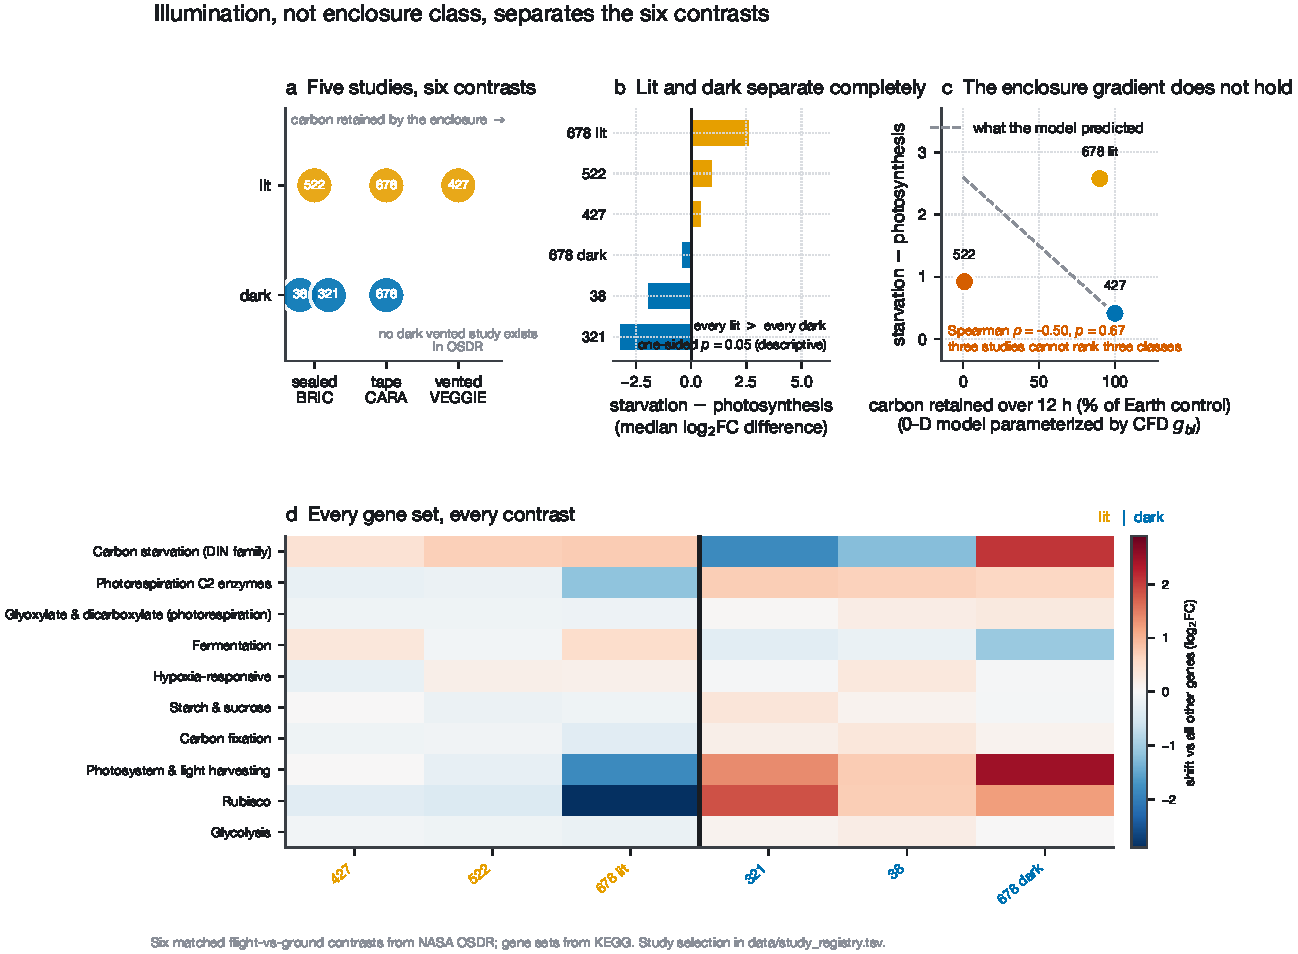
\includegraphics[width=0.52\textwidth]{fig07_hardware_ladder.pdf}\hfill
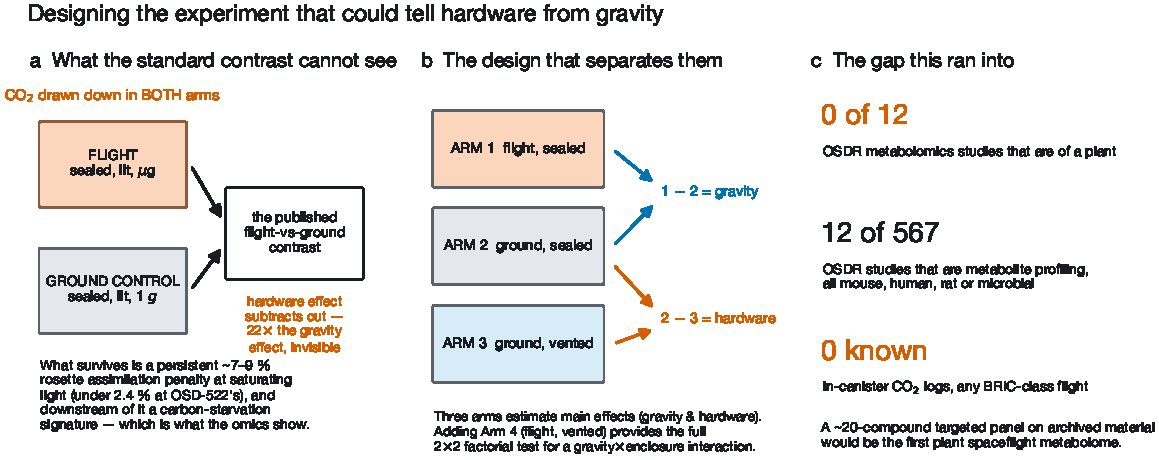
\includegraphics[width=0.46\textwidth]{fig08_implications.pdf}
\caption{\textbf{Cross-study evaluation across six OSDR flight contrasts and experimental design to unconfound hardware from microgravity.}
\textbf{Left} (\texttt{fig07\_hardware\_ladder.pdf}): \textbf{a}, Matrix of six flight-versus-ground contrasts across five OSDR studies. \textbf{b}, Illumination separates all three lit contrasts ($+0.41$, $+0.92$, $+2.58$) from all three dark contrasts ($-0.39$, $-1.95$, $-3.22$; one-sided Mann--Whitney $p = 0.05$) on the carbon-starvation (\textit{DIN}) over photosynthesis contrast (\texttt{T12\_ladder\_contrasts.tsv}). \textbf{c}, Among lit studies, the predicted monotonic gradient across enclosure classes does not hold ($\rho = -0.50$, $p = 0.67$), with dimly lit CARA (\texttt{OSD-678}, $4\text{--}6\,\ums$) sitting highest. \textbf{d}, Heatmap of Mann--Whitney shifts across all ten evaluated gene sets (\texttt{T11\_hardware\_ladder.tsv}).
\textbf{Right} (\texttt{fig08\_implications.pdf}): \textbf{a}, Why standard two-arm spaceflight designs (sealed flight vs.\ sealed ground) cancel the $22\times$ hardware starvation effect while measuring microgravity in carbon-starved plants. \textbf{b}, Proposed three-arm (adding vented ground) and $2\times 2$ factorial (adding vented flight) designs that separate main effects of enclosure atmosphere, microgravity, and their interaction. \textbf{c}, Summary of the OSDR plant metabolomics and in-canister logging archive gaps.}
\label{fig:ladder_implications}
\end{figure*}

Evaluating the ten gene sets and set-versus-set contrasts across all six studies (\texttt{T11\_hardware\_ladder.tsv}, \texttt{T12\_ladder\_contrasts.tsv}; Fig.~\ref{fig:ladder_implications} left) revealed two sharp empirical findings:
\begin{enumerate}
    \item \textbf{Illumination completely separates the six spaceflight contrasts}: On the primary carbon-starvation-over-photosynthesis contrast ($\text{\textit{DIN}} - \text{photosynthesis apparatus}$), \textbf{every illuminated contrast is positive} ($+0.41$ in VEGGIE OSD-427, $+0.92$ in BRIC-LED OSD-522, and $+2.58$ in lit CARA OSD-678) and \textbf{every dark contrast is negative} ($-0.39$ in dark BRIC OSD-38, $-1.95$ in dark BRIC OSD-321, and $-3.22$ in dark CARA OSD-678; descriptive one-sided Mann--Whitney $p = 0.05$; Fig.~\ref{fig:ladder_implications}b). This separation is physically consistent with our central mechanism: photosynthetic $\mathrm{CO_2}$ drawdown and boundary-layer $\mathrm{CO_2}$ depletion require light; in darkness, respiration releases $\mathrm{CO_2}$ rather than consuming it.
    \item \textbf{The simple one-dimensional ranking across enclosure classes does not hold}: Among the three illuminated contrasts, sealed BRIC-LED ($+0.92$) sits above ventilated VEGGIE ($+0.41$) as predicted, but the dimly lit CARA plates in OSD-678 ($+2.58$, grown in only $4\text{--}6\,\ums$ of ambient cabin light near the light compensation point, and with unrecorded plate-sealing tape geometry in OSDR) sit highest (Spearman $\rho = -0.50$, $p = 0.67$; Fig.~\ref{fig:ladder_implications}c).
\end{enumerate}

%=============================================================================
\section*{Discussion}\label{sec:discussion}
%=============================================================================

\subsection*{Two distinct physical scales of gas transport in spaceflight plant biology}

By uniting a validated 2-D lattice-Boltzmann fluid and mass-transport solver with a mechanistic FvCB Rubisco model and testing their combined predictions across NASA OSDR, this study resolves a longstanding ambiguity in spaceflight plant biology. Two distinct transport bottlenecks operate simultaneously in orbital plant experiments, but at different spatial scales and with different consequences for differential multi-omics:
\begin{enumerate}
    \item \textbf{The microgravity boundary layer ($\sim 0.7\text{--}11\,\mathrm{mm}$, $C_a \to C_s$)} is a genuine gravity effect. Eliminating buoyancy-driven convection reduces $g_{bl}$ by $2.0\text{--}2.3\times$ across single leaves, rosettes, and canopies (Table~\ref{tab:cfd_sweep}). At ambient $\mathrm{CO_2}$ ($400\,\mathrm{ppm}$) and moderate-to-high irradiance, this boundary-layer thickening depresses chloroplastic $C_c$, elevates Rubisco oxygenation $\varphi$, and reduces net assimilation by $5\text{--}9\%$ in leaves/rosettes and $26\text{--}29\%$ in dense microgreen canopies (or $<3\%$ and $11\%$ at $60\,\ums$; Fig.~\ref{fig:fvcb}c). Because this penalty is purely diffusive, horizontal forced ventilation of $\approx 2.0\,\cmsu$ (single leaf) to $\approx 6.1\,\cmsu$ (rosette) completely restores Earth-equivalent boundary-layer conductance (Fig.~\ref{fig:fan_scale}).
    \item \textbf{Enclosure headspace drawdown ($10^1\text{--}10^2\,\mathrm{mm}$, $C_{\text{cabin}} \to C_a$)} is a hardware effect. In an illuminated, hermetically sealed canister such as BRIC-LED, photosynthetic uptake exhausts the $\sim 400\,\mathrm{ppm}$ headspace $\mathrm{CO_2}$ to the compensation point in $\sim 7\,\mathrm{min}$, slashing 12\,h carbon gain to $\approx 1\%$ of an unenclosed control and driving Rubisco oxygenation $\varphi$ from $18\%$ to $46\%$ (Fig.~\ref{fig:hardware}, Fig.~\ref{fig:fvcb}). This enclosure effect is $\approx 22\times$ larger than the microgravity boundary-layer effect, and because it is a volume mass balance, it occurs in the $1\,g$ ground control canister just as rapidly as in flight.
\end{enumerate}

This interaction explains why the microgravity boundary-layer penalty and canister carbon starvation cannot be treated as simple additive stresses. As canister $\mathrm{CO_2}$ falls toward the compensation point, net assimilation $A$ approaches zero, so the concentration drop across the boundary layer ($\Delta C_{bl} = A/g_{bl}$) vanishes and the $1\,g$ and $\mu g$ operating points converge (Fig.~\ref{fig:fvcb}b). Likewise, inside a sealed BRIC Petri dish, transpirational humidification saturates the shallow $7.4\,\mathrm{mm}$ headspace within $1\text{--}2\,\mathrm{min}$, extinguishing solutal buoyancy at $1\,g$ so that even the physical conductances $g_{bl}(1\,g)$ and $g_{bl}(0\,g)$ converge (Supplementary Fig.~\ref{fig:s_dish_feedback}). Consequently, a flight-versus-ground comparison in illuminated sealed hardware measures the residual effect of microgravity inside plants that their own growth canister has already severely carbon-starved (Fig.~\ref{fig:ladder_implications} right). Consistent with this transport-limited framework, whole-stand gas exchange of wheat in microgravity is indistinguishable from $1\,g$ at saturating $\mathrm{CO_2}$ \citep{monje2005}---the exact regime in which boundary-layer and enclosure $\mathrm{CO_2}$ limitations are relieved.

\subsection*{What the model explains in the spaceflight multi-ome, and what it does not}

In OSD-522 (BRIC-LED), the coupled model accurately predicted eight of nine directional gene-set shifts in the transcriptome and four of seven in the proteome, including concerted repression of photosystems, Rubisco, Calvin-cycle enzymes, and starch/sucrose synthesis, strong induction of \textit{DIN6/ASN1} carbon-starvation markers, and selective preservation of photorespiratory enzymes relative to Rubisco ($+0.239\,\log_2\mathrm{FC}$ in RNA-seq, $+0.285$ in proteomics; Table~\ref{tab:falsification}). Across five independent OSDR experiments (six matched contrasts), illumination completely separated all lit contrasts from all dark contrasts on the starvation-over-photosynthesis axis (Fig.~\ref{fig:ladder_implications}b).

Equally important are the three places where the data falsified or exceeded the gas-transport model:
\begin{enumerate}
    \item \textbf{Dominance of the endoplasmic reticulum unfolded protein response (UPR)}: The single strongest pathway enrichment in OSD-522 is ER protein processing (\texttt{ath04141}, $p = 8.6\times 10^{-9}$; Fig.~\ref{fig:paintomics}b), a conserved spaceflight stress signature also highlighted in OSD-321 \citep{osd321} that leaf gas transport does not explain. Biophysical and metabolic models of spaceflight adaptation must therefore treat ER proteostasis alongside gas transport rather than assuming gas exchange explains all stress responses.
    \item \textbf{Absence of broad photorespiratory induction in the multi-ome}: While our initial steady-state hypothesis predicted elevated photorespiratory enzymes, the OSD-522 data showed only relative preservation above Rubisco, not absolute induction (Fig.~\ref{fig:osd522_blind}). This matches our coupled FvCB finding: because canister $\mathrm{CO_2}$ exhaustion converges the $1\,g$ and $\mu g$ boundary layers, the differential flux between flight and ground vanishes.
    \item \textbf{Non-monotonicity across lit hardware}: Dimly lit CARA plates in OSD-678 showed a stronger starvation-over-photosynthesis ratio ($+2.58$) than sealed BRIC-LED ($+0.92$), likely because the low $4\text{--}6\,\ums$ irradiance placed the seedlings near the light compensation point while unrecorded tape wrapping may have restricted diffusion.
\end{enumerate}

\subsection*{Recommendations for future spaceflight plant experiments}

Based on these findings, we propose three concrete recommendations to unconfound enclosure atmosphere from microgravity in future orbital plant biology (Fig.~\ref{fig:ladder_implications} right):
\begin{enumerate}
    \item \textbf{Mandatory in-canister environmental logging}: Every spaceflight growth container should log in-dish $\mathrm{CO_2}$, $\mathrm{O_2}$, relative humidity, and PAR at $\ge 1\,\mathrm{min}$ resolution. Without internal atmospheric data, investigators cannot determine whether transcriptional shifts reflect microgravity or enclosure carbon starvation.
    \item \textbf{Targeted 20-compound metabolomics profiling}: NASA and international flight programs should prioritize chemical profiling of archived and future spaceflight plant tissues, targeting the 20 central-carbon and photorespiratory compounds identified here (Fig.~\ref{fig:metabolome}) to close the complete plant metabolomics gap in OSDR.
    \item \textbf{Three-arm and $2\times 2$ factorial experimental designs}: Future flight investigations should move beyond simple two-arm designs (flight vs.\ ground in identical sealed hardware) to three-arm designs (adding an open/vented ground control) or fully crossed $2\times 2$ designs ($\{\text{sealed, vented}\} \times \{\mu g, 1\,g\}$; Fig.~\ref{fig:ladder_implications}b) that explicitly unconfound enclosure atmosphere from microgravity.
\end{enumerate}

%=============================================================================
\section*{Methods}\label{sec:methods}
%=============================================================================

\subsection*{Lattice-Boltzmann solver architecture and governing equations}

The two-dimensional fluid-dynamics engine was implemented in TypeScript and Python using a standard D2Q9 lattice for fluid velocity and three independent D2Q5 lattices for scalar species transport ($\mathrm{CO_2}$, $\mathrm{O_2}$, $\mathrm{H_2O}$). Fluid collision follows the Bhatnagar--Gross--Krook (BGK) relaxation model with a Guo body force \citep{guo2002}:
\begin{equation}
f_i(\mathbf{x} + \mathbf{c}_i\Delta t, t + \Delta t) = f_i(\mathbf{x}, t) - \frac{1}{\tau_f}\left[f_i(\mathbf{x}, t) - f_i^{\text{eq}}(\mathbf{x}, t)\right] + F_i\Delta t ,
\end{equation}
where $\mathbf{c}_i$ are the D2Q9 lattice velocities, $\tau_f$ is the non-dimensional kinematic relaxation time ($\nu = c_s^2(\tau_f - 0.5)\Delta t$), $c_s = 1/\sqrt{3}$ is the lattice speed of sound, and the equilibrium distributions $f_i^{\text{eq}}$ are given by the standard second-order expansion:
\begin{equation}
f_i^{\text{eq}} = w_i\rho\left[1 + \frac{\mathbf{c}_i\cdot\mathbf{u}}{c_s^2} + \frac{(\mathbf{c}_i\cdot\mathbf{u})^2}{2c_s^4} - \frac{\mathbf{u}\cdot\mathbf{u}}{2c_s^2}\right] .
\end{equation}
Body force coupling incorporates solutal and thermal Boussinesq buoyancy:
\begin{equation}
\mathbf{F} = \rho\,\mathbf{g}\left[-\beta_{\mathrm{H_2O}}\Delta C_{\mathrm{H_2O}} + \beta_{\mathrm{CO_2}}\Delta C_{\mathrm{CO_2}} - \beta_T\Delta T\right] ,
\end{equation}
where $\beta_k = (M_{\text{air}} - M_k)/M_{\text{air}}$ is the solutal expansion coefficient ($\beta_{\mathrm{H_2O}} = (28.97 - 18.015)/28.97 = +0.378$ for buoyant water vapour; $\beta_{\mathrm{CO_2}} = (28.97 - 44.01)/28.97 = -0.519$ for heavy $\mathrm{CO_2}$). Species transport on D2Q5 follows:
\begin{multline}
g_{k,j}(\mathbf{x} + \mathbf{e}_j\Delta t, t + \Delta t) = g_{k,j}(\mathbf{x}, t) \\
- \frac{1}{\tau_{s,k}}\left[g_{k,j}(\mathbf{x}, t) - g_{k,j}^{\text{eq}}(\mathbf{x}, t)\right] + S_{k,j}\Delta t ,
\end{multline}
where $\mathbf{e}_j$ are the five discrete velocity vectors, $D_k = c_{s,5}^2(\tau_{s,k} - 0.5)\Delta t$, and $S_{k,j}$ denotes stomatal source/sink terms applied at leaf boundary nodes. Mid-grid bounce-back boundary conditions were enforced at solid walls and leaf surfaces. An optional multiple-relaxation-time (MRT) collision operator was implemented in modal space using the Gram--Schmidt orthogonal basis of Lallemand and Luo \citep{lallemand2000}.

\subsection*{Coupled FvCB photosynthesis and Rubisco kinetics}

Steady-state boundary-layer conductances ($g_{bl} = F/\Delta C_s$) obtained from the converged CFD fields were coupled in series with stomatal ($g_s = 0.15\,\molms$) and mesophyll ($g_m = 0.20\,\molms$) conductances to compute the chloroplastic $\mathrm{CO_2}$ mole fraction ($C_c$) under the Farquhar--von Caemmerer--Berry (FvCB) $\mathrm{C_3}$ photosynthesis model \citep{farquhar1980}:
\begin{equation}
A = \min(A_c, A_j) - R_d ,
\end{equation}
\begin{equation}
A_c = \frac{V_{c\max}(C_c - \Gamma^*)}{C_c + K_c(1 + O_c/K_o)}, \qquad A_j = \frac{J(C_c - \Gamma^*)}{4C_c + 8\Gamma^*} ,
\end{equation}
where $V_{c\max} = 60\,\ums$, $J_{\max} = 120\,\ums$, $K_c = 404\,\mu\mathrm{mol\,mol^{-1}}$, $K_o = 248\,\mathrm{mmol\,mol^{-1}}$, $\Gamma^* = 42.75\,\mu\mathrm{mol\,mol^{-1}}$, and $R_d = 1.18\,\ums$ at $25\,^\circ\mathrm{C}$ \citep{bernacchi2001,bernacchi2003}. Rubisco oxygenation rate and oxygenation fraction were computed explicitly:
\begin{align}
V_c &= \frac{A + R_d}{1 - \Gamma^*/C_c}, \qquad V_o = \frac{2\Gamma^*}{C_c}V_c, \\
\varphi &= \frac{V_o}{V_o + V_c} = \frac{2\Gamma^*}{C_c + 2\Gamma^*} .
\end{align}
The supply-side mass balance $A = g_{tc}(C_a - C_c)$ (where $g_{tc}^{-1} = g_{bl}^{-1} + g_s^{-1} + g_m^{-1}$) was solved recursively to machine precision using Brent's method.

\subsection*{OSDR data acquisition, processing, and PaintOmics 4 integration}

Unnormalized RSEM gene-level counts for OSD-522 ($n=6$ flight, $n=6$ ground shoot libraries) were retrieved via the NASA OSDR API (\texttt{scripts/00\_fetch\_osdr.py}) and analyzed with PyDESeq2 \citep{pydeseq2} (\texttt{scripts/01\_dge\_rnaseq.py}) using design $\sim\texttt{condition}$ with Cook's distance outlier refitting and independent filtering (\texttt{T01\_osd522\_transcriptome.tsv}). Deposited TMT soluble and membrane shoot proteomics tables from OSD-522 were merged by UniProt/AGI accession (\texttt{scripts/02\_prep\_proteomics.py}, \texttt{T02\_osd522\_proteome.tsv}). Gene sets (\texttt{scripts/genesets.py}) were retrieved live from the KEGG REST API \citep{kanehisa2000,kegg} (\texttt{ath00630}, \texttt{ath00710}, \texttt{ath00500}, \texttt{ath00010}, \texttt{ath00195}, \texttt{ath00196}) alongside curated Araport11 locus sets for core photorespiratory enzymes (\texttt{photorespiration\_core}, $n=13$), Rubisco ($n=5$), \textit{DIN} carbon-starvation markers ($n=5$), fermentation ($n=6$), and core hypoxia markers ($n=3$). Directional falsification tests (\texttt{scripts/04\_falsification\_check.py}) used two-sided Mann--Whitney $U$ tests of gene-set $\log_2\mathrm{FC}$ distributions against the genome-wide background (\texttt{T07\_falsification\_osd522.tsv}). Multi-omics pathway enrichment was performed in PaintOmics 4 \citep{paintomics4} across KEGG and MapMan ontologies (saved job record \texttt{oK2h66740Q}, verified against metabolite-free control \texttt{T17\_integration\_control\_nometa.tsv} and external Fisher/Mann--Whitney tests \texttt{T16\_independent\_pathways.tsv}). MapMan pathway membership (\texttt{scripts/mapman.py}) was reconstructed deterministically from GoMapMan Araport11 bin assignments and vendored MapManStore diagram layouts (\texttt{data/mapman/PROVENANCE.md}). Cross-study evaluation (\texttt{scripts/07\_hardware\_ladder.py}) ingested GeneLab differential expression tables for OSD-522, OSD-38, OSD-321, OSD-678, and OSD-427 according to the audit rules in \texttt{data/study\_registry.tsv}.

\subsection*{Use of AI coding and drafting assistants}

In accordance with publisher guidelines on artificial intelligence transparency, the author discloses that AI coding and drafting assistants (Claude Code, Anthropic; Google Antigravity) were used under the author's direct supervision to implement solver and pipeline scripts, generate figures, and format manuscript drafts. The author independently verified all physical equations, numerical validation gates, OSDR data processing, statistical tests, and bibliographic citations, and takes full responsibility for the integrity of the work.

%=============================================================================
\section*{Data Availability}
%=============================================================================

All source code (TypeScript/React 2-D lattice-Boltzmann CFD workbench, headless validation suite, Python FvCB and multi-omics pipeline, and interactive web applications), derived tables (\texttt{T1}--\texttt{T24} and \texttt{T01}--\texttt{T17} with machine-verified provenance in \texttt{results/MANIFEST.tsv}), publication figures, and LaTeX/Word manuscript sources are openly available at \url{https://github.com/dr-richard-barker/Spaceflight-Plant-Biophysics-Multiomics} under the MIT (code) and CC-BY-4.0 (manuscript and figures) licenses, and archived on Zenodo. Primary spaceflight multi-omics datasets are publicly available in the NASA Open Science Data Repository \citep{osdr2025} under accessions OSD-522 \citep{osd522}, OSD-38 \citep{osd38}, OSD-321 \citep{osd321}, OSD-678 \citep{osd678}, and OSD-427 \citep{osd427}. Empirical whole-plant chamber gas-exchange data from Chew et al.~\citep{chew2022} are archived at Edinburgh DataShare (\url{https://doi.org/10.7488/ds/3453}) \citep{chew2022data}.

%=============================================================================
\section*{Code Availability}
%=============================================================================

The complete computational codebase is open-source and version-controlled at \url{https://github.com/dr-richard-barker/Spaceflight-Plant-Biophysics-Multiomics}. The browser-based 2-D CFD simulation workbench and the interactive FvCB and multi-omics explorer are hosted live via GitHub Pages at \url{https://dr-richard-barker.github.io/Spaceflight-Plant-Biophysics-Multiomics/}.

%=============================================================================
\section*{References}
%=============================================================================

\bibliographystyle{naturemag}
\bibliography{references}

%=============================================================================
\section*{Acknowledgements}
%=============================================================================

The author thanks Y.~H. Chew and A.~J. Millar (University of Edinburgh) for open whole-plant chamber gas-exchange datasets, the NASA Open Science Data Repository (OSDR / GeneLab) team and Analysis Working Groups, and the spaceflight plant biology investigators who generated the archival flight datasets analyzed here.

%=============================================================================
\section*{Author Contributions}
%=============================================================================

\textbf{R.J.B.} conceived the study, developed the lattice-Boltzmann CFD solver, formulated the coupled FvCB and metabolite models, processed the NASA OSDR datasets, executed the multi-omics integration and statistical evaluations, generated all figures and tables, and wrote the manuscript.

%=============================================================================
\section*{Competing Interests}
%=============================================================================

The author declares no competing financial or non-financial interests.

%=============================================================================
\section*{Additional Information}
%=============================================================================

\textbf{Supplementary information} is available for this paper at \url{https://dr-richard-barker.github.io/Spaceflight-Plant-Biophysics-Multiomics/Spaceflight_Biophysics_Multiomics_SI.pdf}.

\textbf{Correspondence and requests for materials} should be addressed to R.J.B. (\href{mailto:dr.richard.barker@gmail.com}{dr.richard.barker@gmail.com}).

\end{document}
